% !TeX TXS-program:compile = txs:///pdflatex/[--shell-escape]
\documentclass[a4paper]{article} \usepackage[backend=biber, style=numeric, sorting=none]{biblatex}
\usepackage[a4paper, left=0.8cm, right=0.8cm, top=0.8cm, bottom=0.8cm, landscape]{geometry}
\usepackage{multicol}
\usepackage{blindtext}
\usepackage{listings}
\usepackage{graphicx}
\usepackage{enumitem}
\usepackage{amssymb}
\usepackage{xcolor}
\usepackage{caption}
\usepackage{mathtools}

\DeclarePairedDelimiter\ceil{\lceil}{\rceil}
\DeclarePairedDelimiter\floor{\lfloor}{\rfloor}

\newenvironment{Figure}
  {\par\medskip\noindent\minipage{\linewidth}}
  {\endminipage\par\medskip}
\renewcommand{\labelitemii}{$\circ$}

\begin{document}
\setlength\parindent{0pt}
\scriptsize
\setlist{nosep}
\setlist[itemize]{leftmargin=*}

\begin{center}
{\large CS2100 Finals Cheatsheet 2021/22 Sem 1}
\end{center}
    \begin{multicols*}{4}

% Boolean Algebra %
{\small\textbf{\textcolor{blue}{Boolean Algebra}}}
\\\\\textbf{Logic Circuit}
\begin{itemize}
\item Advantages of digital circuits over analogue circuit:
    \begin{itemize}
        \item More reliable (simpler circuits, less noise)
        \item Specified accuracy (determinable)
        \item Abstraction can be applied using boolean algebra
        \item Easy design, analysis and simplification of digital circuit
    \end{itemize}
\item \textbf{Combinational}: No memory, output depends solely on input (e.g. gates, decoders, multiplexers, adders and multipliers)
\item \textbf{Sequential}: with memory, output depends on both input and current state (e.g. counters, registers, memories)\\
\end{itemize}

\textbf{Precedence of operators}
\begin{itemize}
\item Precedence from highest to lowest
    \begin{itemize}
        \item Not ($'$)
        \item And ($.$)
        \item Or (+)
    \end{itemize}
\item Use parenthesis to overwrite precedence\\
\end{itemize}

\textbf{Laws}
\begin{itemize}
\item \textbf{Identity}: $A + 0 = A$ and $A \cdot 1 = A$
\item \textbf{Inverse/Complement}: $A + A' = 1$ and $A \cdot A' = 0$
\item \textbf{Commutative}: $A + B = B + A$  and $A \cdot B = B \cdot A$
\item \textbf{Associative}: $A + (B + C) = (A + B) + C$ and $A \cdot (B \cdot C) = (A \cdot B) \cdot C$
\item \textbf{Distributive}: $A + (B \cdot C) = (A + B) \cdot (A + C)$ and $A \cdot (B + C) = (A \cdot B) + (A \cdot C)$
\item \textbf{Duality} (not a real law): If we flip AND/OR operators and flip the operands (0 and 1), the boolean equation still holds\\
\end{itemize}

\textbf{Theorems}
\begin{itemize}
\item Idempotency: $X + X = X$ and $X \cdot X = X$
\item One/Zero Element: $X + 1 = 1$ and $X \cdot 0 = 0$
\item Involution: $(X')' = X$
\item Absorption 1: \\ $X + (X \cdot Y) = X$ \\ $X \cdot (X + Y) = X$
\item Absorption 2: \\ $X + (X' \cdot Y) = X + Y$ \\ $X \cdot (X' + Y) = X \cdot Y$
\item DeMorgan's (can be used on $>2$ variables): \\ $(X \cdot Y)' = X' + Y'$ \\ $(X + Y)' = X' \cdot Y'$
\item Consensus: \\ $(X \cdot Y) + (X' \cdot Z) + (Y \cdot Z) = (X \cdot Y) + (X' \cdot Z)$ \\ $(X + Y) \cdot (X' + Z) \cdot (Y + Z) = (X + Y) \cdot (X' + Z)$\\
\end{itemize}

\textbf{Standard forms}
\begin{itemize}
\item Literals: Boolean variable on its own or in its complemented form (e.g. $X, X', Y, Y'$)
\item Product term: A single literal or a product of several literals (e.g. $X, X\cdot Y\cdot Z', A\cdot B'$)
\item Sum term: A single literal or sum of several literals (e.g. $X, X+Y+Z', A+B'$)
\item Sum-Of-Products (SOP): Product term or a logical sum of product terms (e.g. $X, X + (Y\cdot Z'), X \cdot Y' + X' \cdot Y \cdot Z)$
\item $m$interm: Product term that contains $n$ literals from all the variables (e.g. 2 variable $X$ and $Y$, the minterms are $X'\cdot Y', X'\cdot Y)$
\item Product-Of-Sum (POS): Sum term or a logical product of sum terms (e.g. $X, X \cdot (Y+Z'), (X+Y')\cdot(X'+Y+Z))$
\item $M$axterm: Sum term that contains $n$ literals from all the variables (e.g. On 2 variable $X$ and $Y$, the maxterms are $X'+Y', X'+Y, X+Y')$
\item $Mx$ = $mx'$ because of De Morgan's
\item In general, with $n$ variables we have up to $2^n$ minterms and $2^n$ maxterms
\item Sum of 2 distinct Maxterms is 1 e.g $M1234 + M1120 = 1$
\item Product of 2 distinct minterms is 0 e.g $m1234 \cdot m1120 = 0$\\

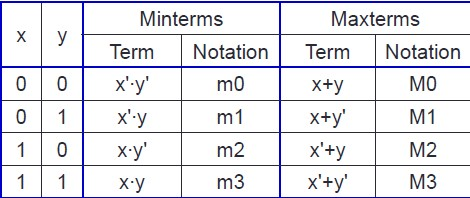
\includegraphics[scale=0.5]{min_max_terms.jpg}\\

\item \textbf{NOTE: $XOR$ = $A'\cdot B + A\cdot B'$ OR $A+B \cdot A'+B'$}
\end{itemize}

{\small\textbf{\textcolor{blue}{Logic Circuits}}}
\\\\\textbf{Gates}

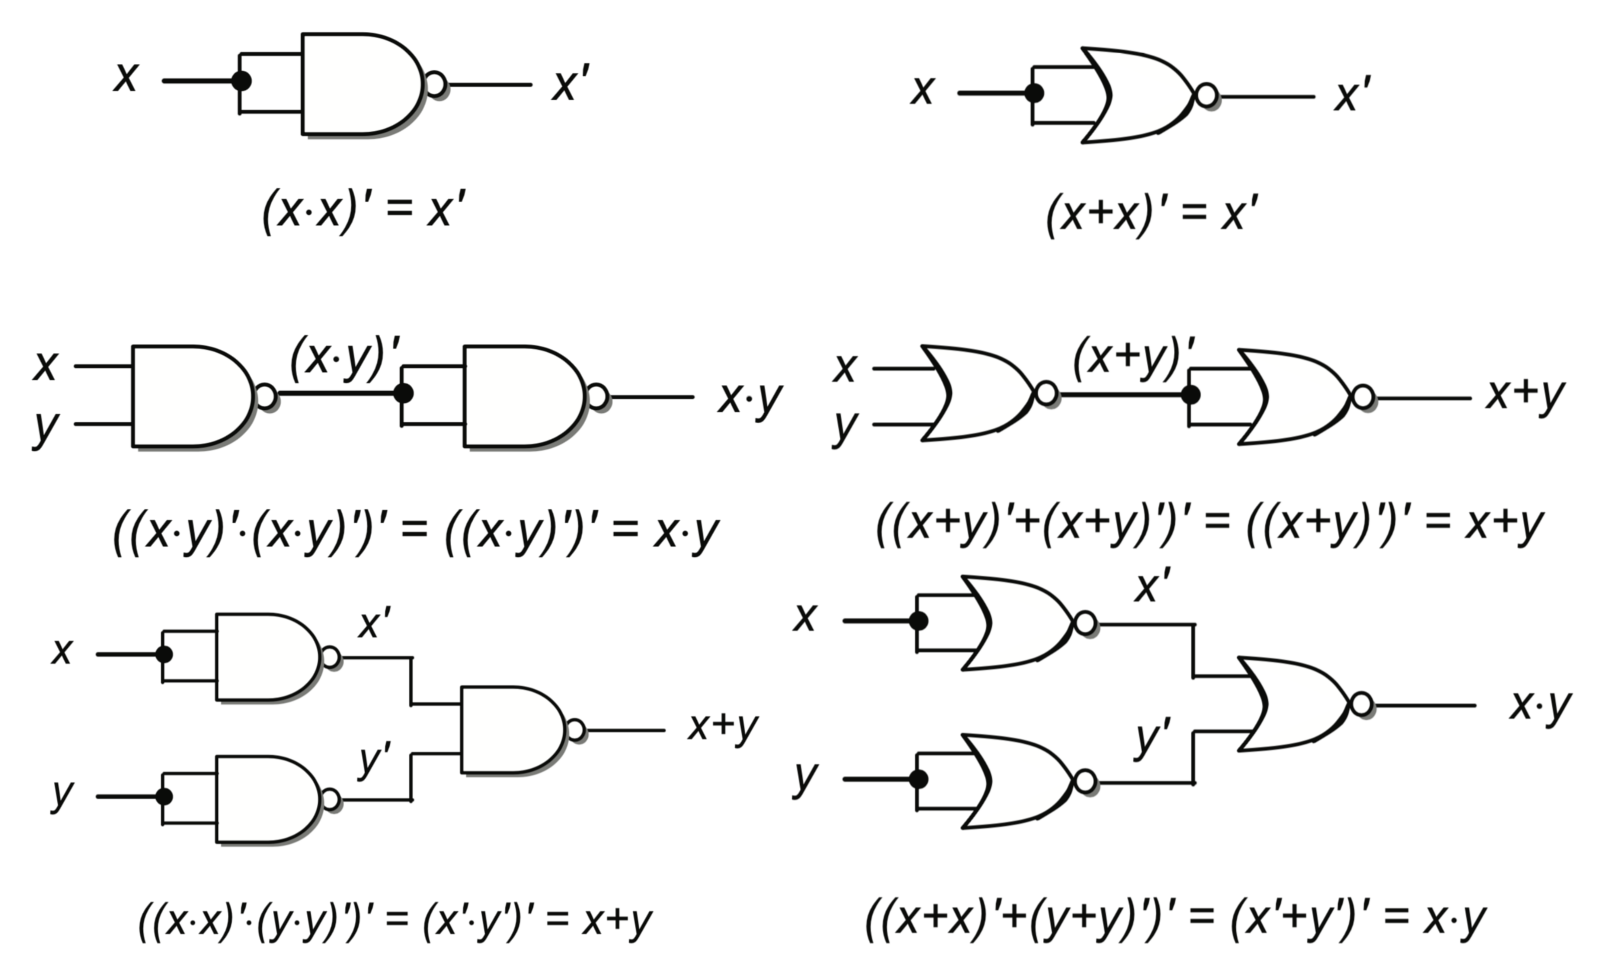
\includegraphics[scale=0.1]{nor_nand.png}

\begin{itemize}
\item {AND, OR, NOT} is a complete set of logic
\item {NAND} is a complete set of logic
\item {NOR} is a complete set of logic
\item SOP can be implemented with 2-level $AND-OR$ circuit or 2-level $NAND$ circuit

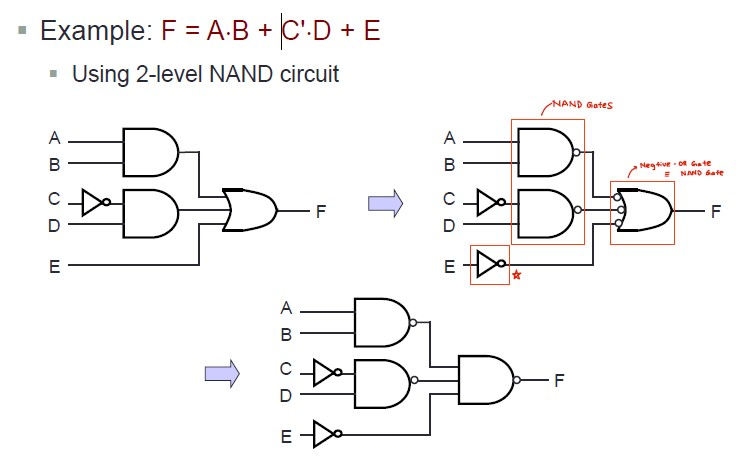
\includegraphics[scale=0.35]{SOP_NAND.jpg}
\vspace{1mm}
\columnbreak
\item POS can be implemented with 2-level $OR-AND$ circuit or 2-level $NOR$ circuit
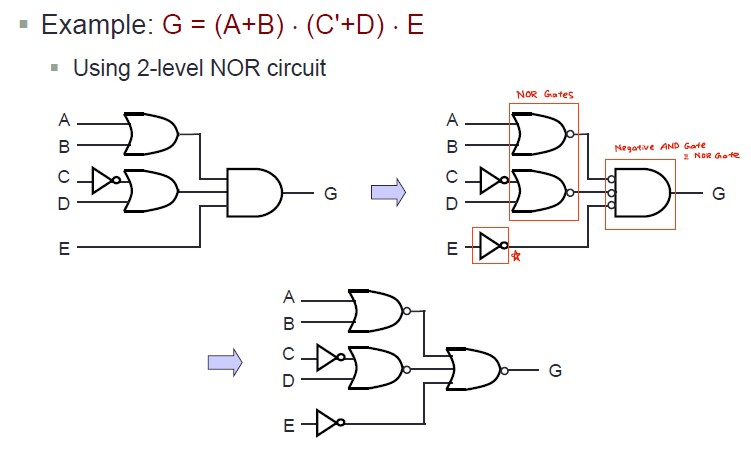
\includegraphics[scale=0.35]{POS_NOR.jpg}
\item With negated outputs, use NAND to simulate OR and NOR to simulate AND\\
\end{itemize}

{\small\textbf{\textcolor{blue}{Simplification}}}
\\\\\textbf{Half Adder}\\
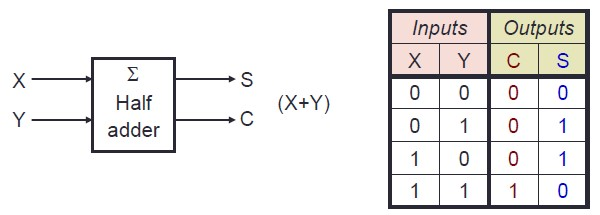
\includegraphics[scale=0.40]{Half_Adder.jpg}
\begin{itemize}
\item $C=X\cdot Y$
\item $S=X'\cdot Y+X\cdot Y' = X\oplus Y$\\
\end{itemize}
\textbf{Gray Code}
\begin{itemize}
    \item Unweighted (not an arithmetic code)
    \item Only a single bit change from one code value to the next
    \item Not restricted to decimal digits: $n$ bits $\rightarrow$ $2^n$ values
    \item Good for error detection
\end{itemize}
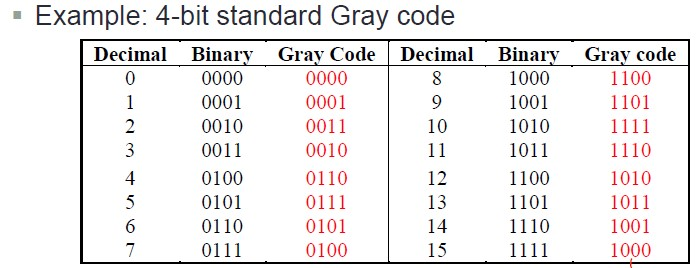
\includegraphics[scale=0.40]{Gray_code.jpg}\\
\textbf{K-Maps}
\begin{itemize}
\item \textbf{Prime Implicant} (PI) is a product term formed by combining the $maximum$ possible no. of minterms (largest group)
\item \textbf{Essential Prime Implicant} (EPI) is a PI that includes at least one minterm not covered by any other group
\item Grouping $2^n$ cells \textcolor{red}{(group must have size in powers of 2)} eliminates n variables
\item Algorithm to finding SOP Expressions
\begin{enumerate}
    \item Circle all prime implicants on the K-map
    \item Identify and select all essential prime implicants for the cover
    \item Select a minimum subset of remaining prime implicants to complete the cover
\end{enumerate}
\item EPIs are counted only by checking 1s, {\bf not} $X$s
\end{itemize}
\columnbreak
{\small\textbf{\textcolor{blue}{Combinatorial Circuits}}}

\textbf{Comparator}\\
compares 2 unsigned values A and B, to check if A>B, A=B, or A<B.
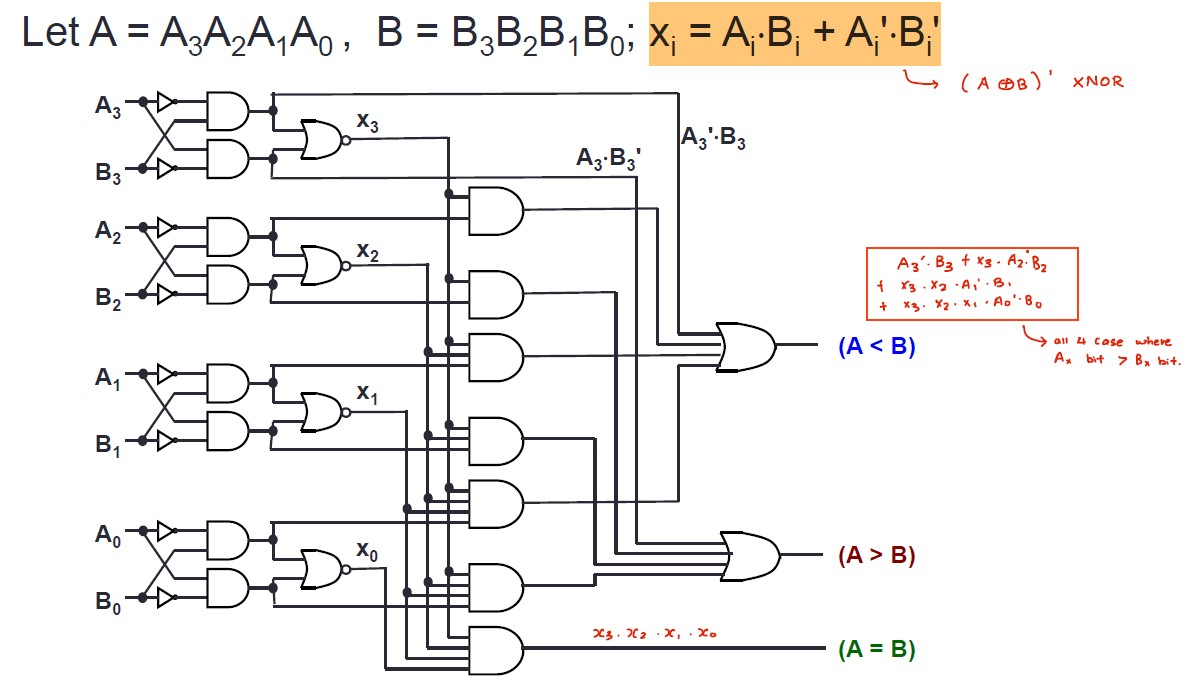
\includegraphics[width=\columnwidth]{comparator}

\textbf{Full Adder}\\
Full adder takes in 3 input (X, Y and Carry in) and returns the number of 1s in the inputs.\\

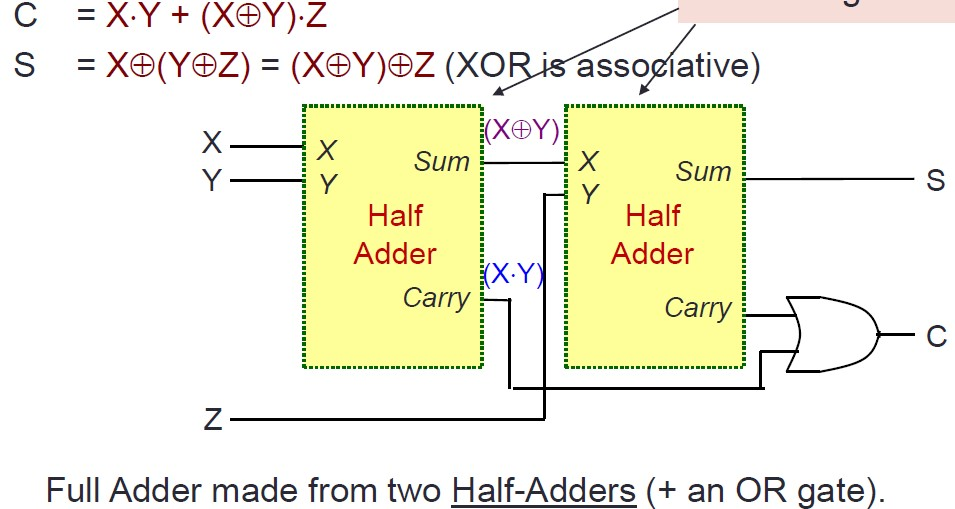
\includegraphics[scale=0.3]{full_adder.jpg}

\textbf{Parallel Adder}\\
Parallel adder adds two 4-bit numbers together and a carry-in, to produce a 5-bit result.\\

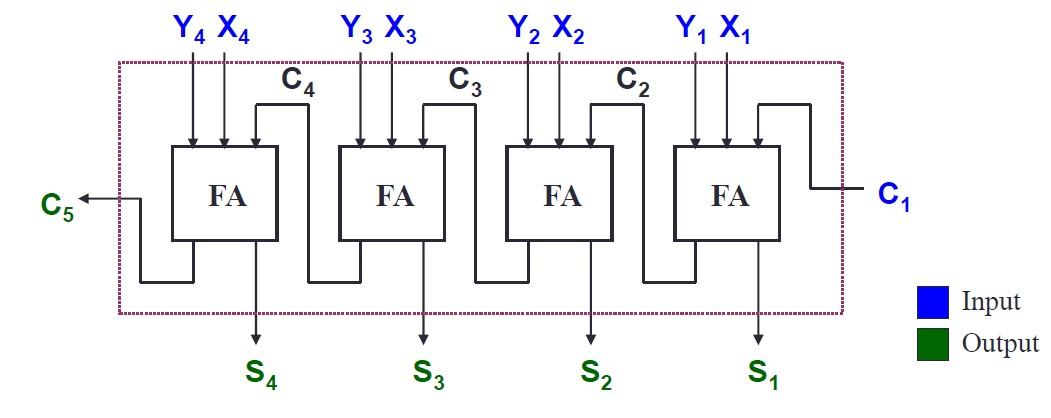
\includegraphics[scale=0.3]{parallel_adder.jpg}

\begin{itemize}
    \item Created by cascading 4 full adders
    \item Carry is propagated by cascading carry from one full adder to the next
\end{itemize}

\columnbreak
\textbf {Delays}: Given a logic gate with delay t, and inputs are stable at times $t_1, t_2, \dots,t_n$, then earliest time where output is stable $ = max(t_1, t_2, \dots t_n) + t$

\begin{Figure}
 \centering
 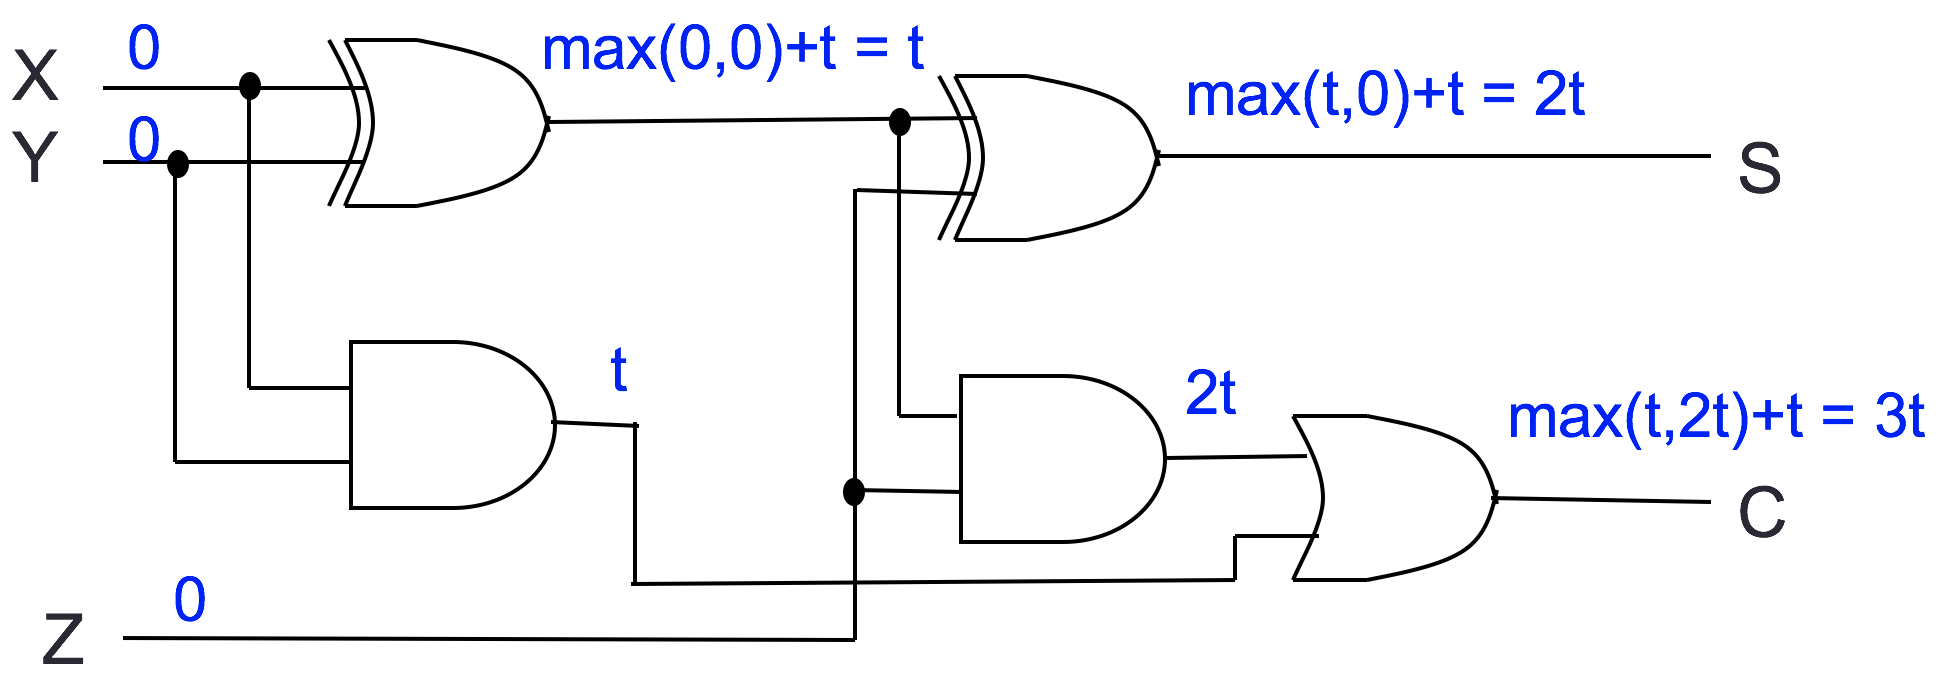
\includegraphics[scale=0.18]{circuit_delay.png}
 \captionof{figure}{Delay of full adder circuit}
\end{Figure}

In general, an $n$-bit ripple carry parallel adder will experience delay of: \textcolor{red}{$S_n = (2(n-1)+2)t, C_{n+1}=(2(n-1)+3)t$ and a maximum delay of $(2(n-1)+3)t$}\\

{\small\textbf{\textcolor{blue}{MSI Components}}}
\begin{multicols*}{2}
\textbf{{Decoder}}
\begin{itemize}
    \item Convert binary information from $n$ input lines to (a maximum of) $2^n$ output lines
    \item Generates $2^n$ minterms of $n$ input variables
    \item Can be used to implement functions by generating minterms using \textcolor{red}{active high} decoder and using an $OR$ gate to form a sum-of-minterm, or a $NOR$ gate to form a product-of-maxterms function
\end{itemize}
\columnbreak

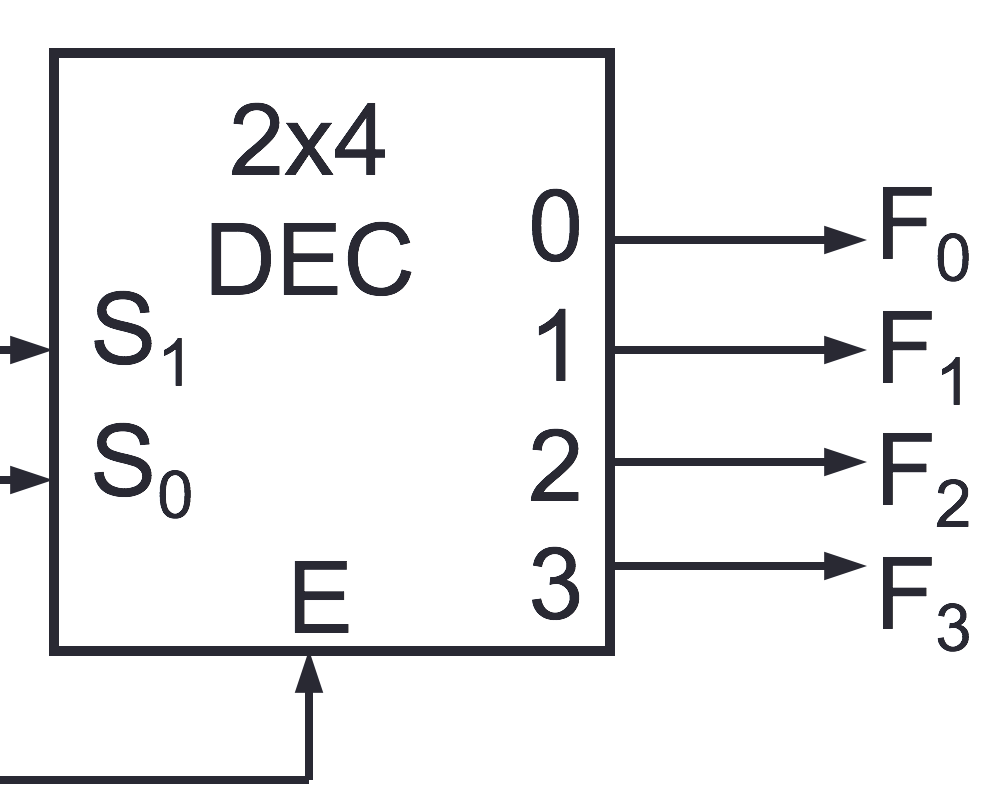
\includegraphics[width=1\columnwidth]{decoder}
\textbf{Note:} When enable is 0 for \textcolor{red}{one-enable} decoder, all output will be 0.
\end{multicols*}

\begin{multicols*}{2}
\textbf{{Encoder}}
\begin{itemize}
    \item Encoding is the converse of decoding $\rightarrow$ Given a set of input lines, of which only one is high, encoder provides a code that corresponds to input line
    \item Contains $2^n$ input lines and $n$ output lines and is implemented with $OR$ gates
\end{itemize}
\columnbreak

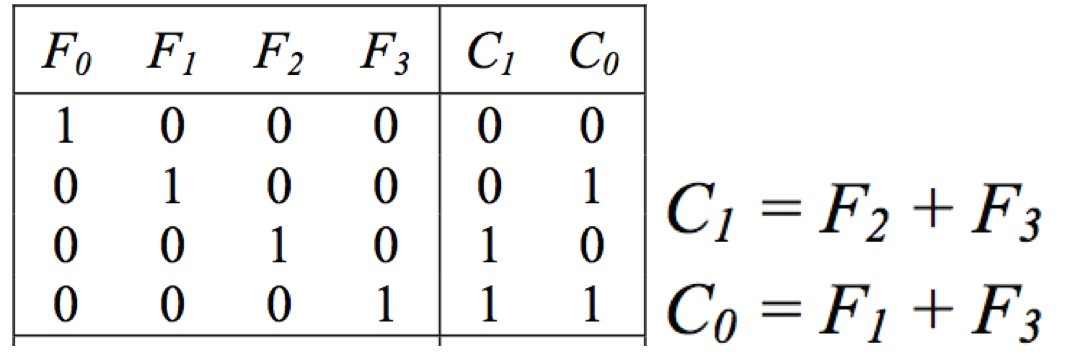
\includegraphics[width=1\columnwidth]{encoder}

\end{multicols*}

\begin{multicols*}{2}
\textbf{{Priority Encoder}}\\
\textbf{Note:} If all inputs are 0, the input combination is considered \textcolor{red}{invalid}
\columnbreak

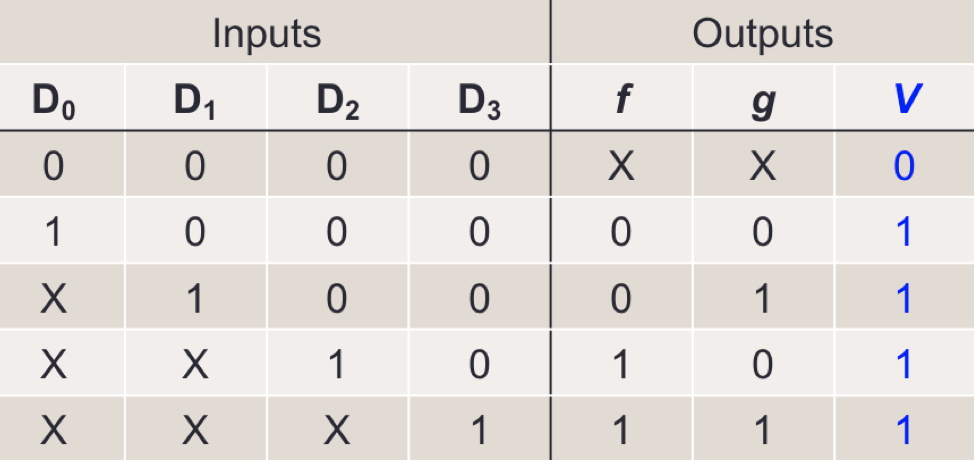
\includegraphics[width=1\columnwidth]{priorityEncoder}
\end{multicols*}

\begin{multicols*}{2}
\textbf{{Multiplexer}}
\\ Use minterm as selection line, using 0/1 as inputs. For smaller size multiplexer, use one of the variables for input lines.
\vfill\null
\columnbreak
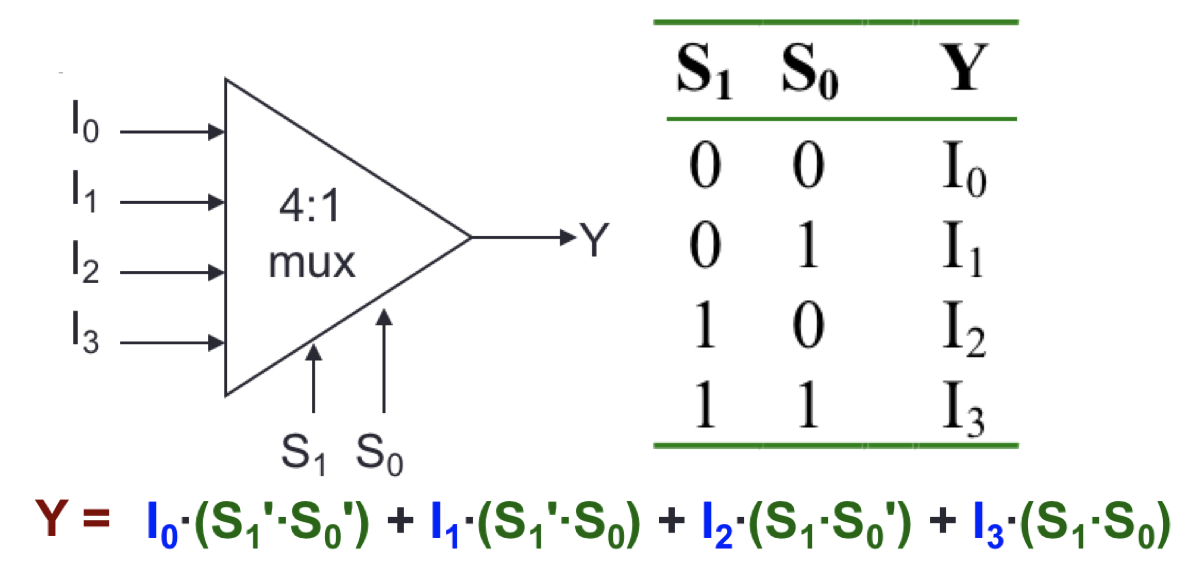
\includegraphics[width=1\columnwidth]{multiplexer}
\end{multicols*}
\columnbreak
\textbf{{Demultiplexer}}
\begin{itemize}
    \item Demultiplexers are identical to decoder with enable
\end{itemize}

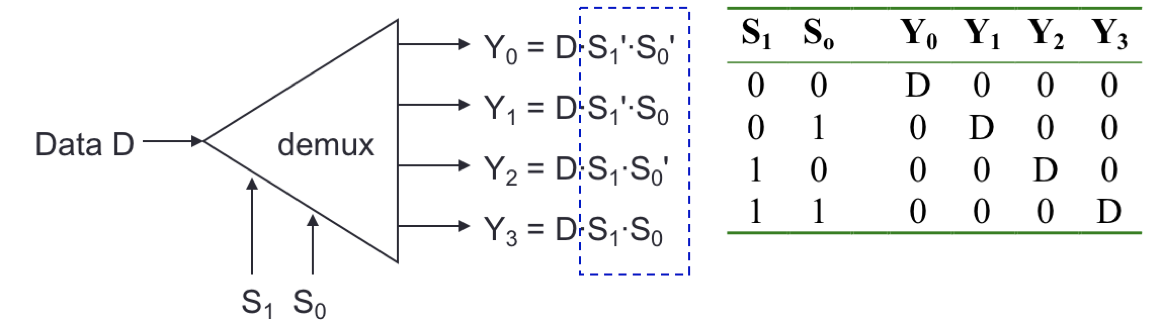
\includegraphics[width=1\columnwidth]{demultiplexer}

%SEQUENTIAL LOGIC%
{\small\textbf{\textcolor{blue}{Sequential Logic}}}
\\\\\textbf{{Two types of sequential circuits}}
\begin{itemize}
    \item \textcolor{blue}{Synchronous}: Outputs change only at specific time
    \item \textcolor{blue}{Asynchronous}: Outputs change at any time\\
\end{itemize}

\textbf{Self-correcting circuit\\}
From \underline{any} unused state, a circuit is able to transition to a valid (used) state after finite number of transitions\\

\textbf{S-R Latch}
\begin{itemize}
    \item Asynchronous device
    \item When $Q=HIGH$, latch is in \textcolor{red}{SET} state, $Q=LOW$, latch is in \textcolor{red}{RESET} state
    \item \textcolor{red}{Drawback}: Invalid condition exists and must be avoided before circuit is stable
    \item $Q(t+1)=S+R'\cdot Q, \\S\cdot R = 0$
    \begin{center}
    \begin{tabular}{ll|ll}
    S & R & $Q^+$         &           \\ \hline
    0 & 0 & Q(t)          & No change \\
    0 & 1 & 0             & Reset     \\
    1 & 0 & 1             & Set       \\
    1 & 1 & indeterminate &
    \end{tabular}
    \textit{Characteristic table of S-R Latch}
    \end{center}
\end{itemize}
\textbf{D Latch}
\begin{itemize}
    \item Asynchronous device
    \item Similar to S-R latch but make input of R equal to S'
    \item Eliminates the undesirable condition of invalid state in S-R latch
    \item $D=HIGH \rightarrow$ latch is SET, $D=LOW \rightarrow$ latch is RESET
    \item Q "follows" D input
    \begin{center}
    \begin{tabular}{ll|ll}
    EN & D & $Q^+$ &           \\ \hline
    1  & 0 & 0     & Reset     \\
    1  & 1 & 1     & Set       \\
    0  & X & Q(t)  & No change
    \end{tabular}
    \textit{\\Characteristic table of D Latch}
    \end{center}
\end{itemize}
\textbf{Flip-Flops}
\begin{itemize}
    \item Synchronous bi-stable devices
    \item Change state at \textbf{rising edge} or \textbf{falling edge} of clock signal
    \item For $m$ flip-flops, up to $2^m$ states exist.
    \item SR has invalid code while JK uses that for the toggle code
    \item Negative input for $Clock$ $\rightarrow$ flip-flop is negative edge-triggered
    \item J-K Flip-flop: $Q^+=J\cdot Q' + K'\cdot Q$
    \item T Flip-flop: $Q^+ = T\cdot Q' + T'\cdot Q$
\end{itemize}
\columnbreak
\textbf{Design and analysis of Sequential Logic}
\begin{itemize}
    \item \textit{Analysis}: Start from circuit diagram $\rightarrow$ derive state table/state diagram
    \item \textit{Design}: Start from a set of specifications (in the form of state equations, table or diagrams) $\rightarrow$ derive logic circuit
    \item \textcolor{blue}{\textit{Characteristic tables}} are use in analysis
    \item \textcolor{red}{\textit{Excitation tables}} are use in analysis
    \item Number of flip-flops needed for $m$ states $=\ceil{log_2(m)}$
    \item Number of input/output:
        \begin{itemize}
            \item Only 1 number tagged to each transition arrow in state diagram $\rightarrow$ 1 input
            \item State diagram shows $/x$ tagged to each transition arrow $\rightarrow$ 1 output
            \item State diagram shows $x/y$ tagged to each transition arrow $\rightarrow$ 1 input, 1 output
        \end{itemize}
\end{itemize}

\textbf{Characteristic table}
\\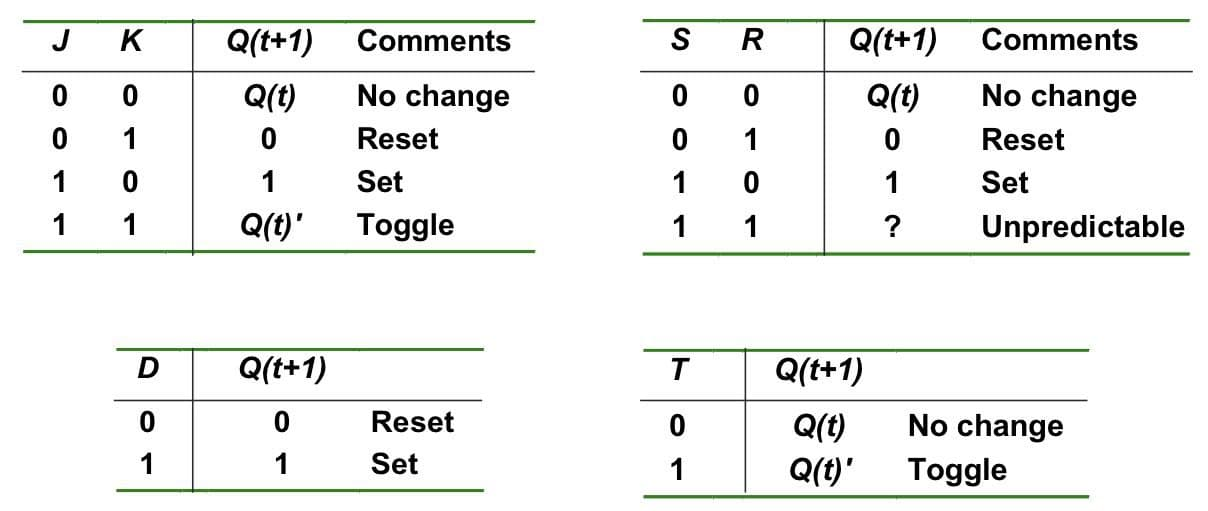
\includegraphics[width=\columnwidth]{flipflops_ct}
\textbf{Excitation Tables}
\\ 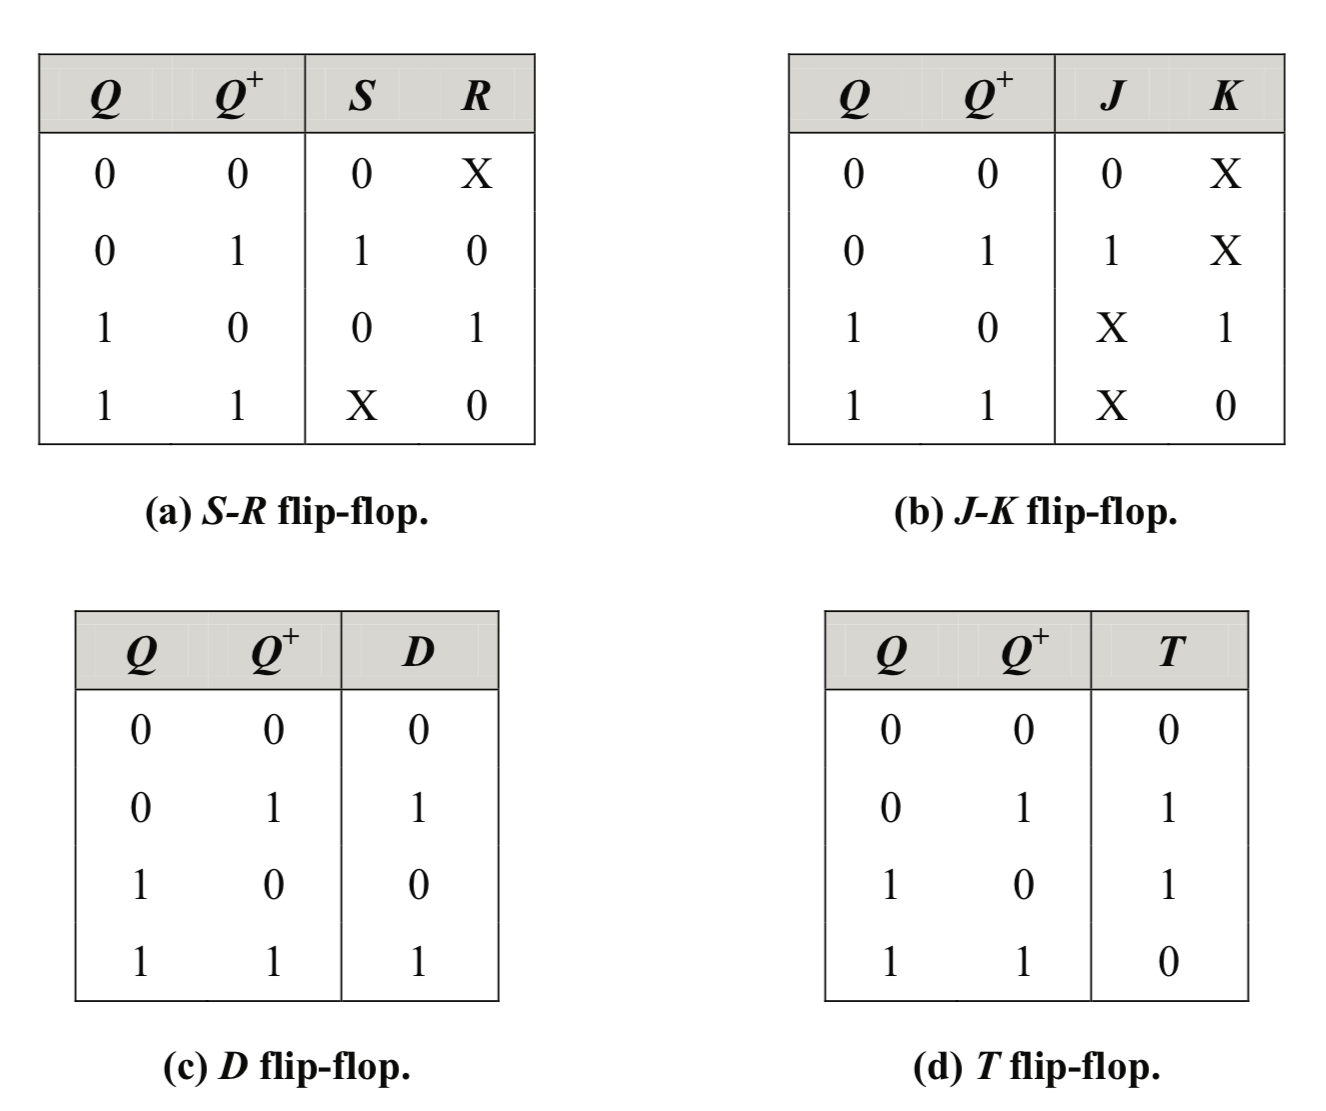
\includegraphics[width=1\columnwidth]{excitationTables}

\textbf{{RAM}}
\\ {\centering 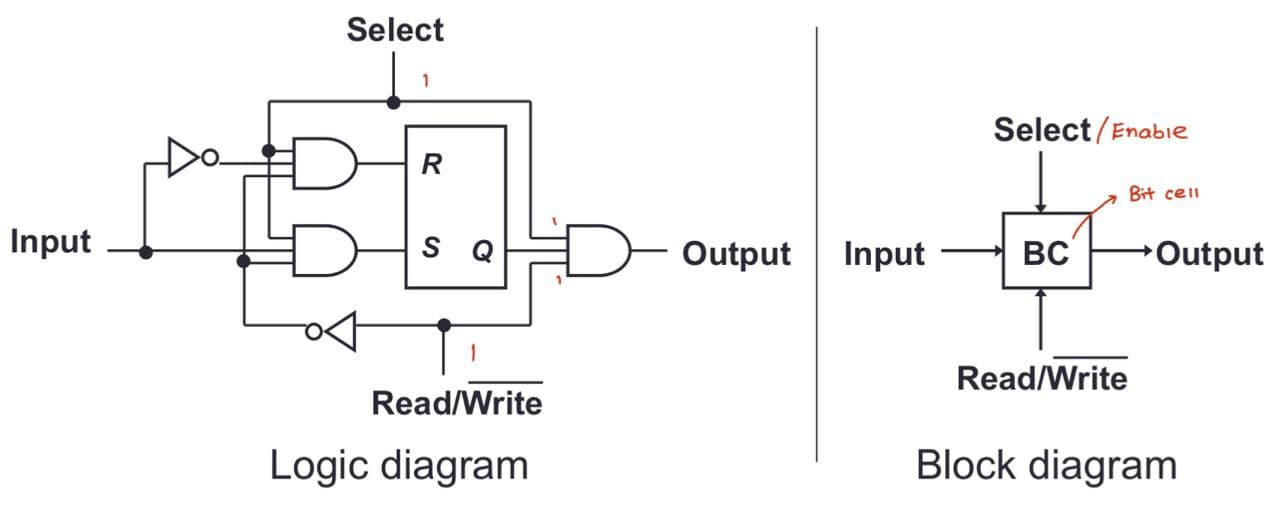
\includegraphics[width=\columnwidth]{staticram.jpg}}
\begin{itemize}
\item Static RAM use flip-flops as memory cells
\item Dynamic RAM uses capacitor charges to represent data, simple in circuitry but have to be constantly refreshed
\item For BC, Write is 0, Read is 1
\item 1K*8 RAM $\Rightarrow$ 1024words*8bits
\item In 12 bit address to 4K*8 RAM constructed using 1K*8 blocks, the 2 most significant bits are fed into decoder to determine which block to use.
\end{itemize}


%PIPELINING%
{\small\textbf{\textcolor{blue}{Pipelining}}}
\\\\ \textbf{Introduction}
\begin{itemize}
    \item Pipelining does not help with latency of single task but it helps with the throughput of entire workout (same amount of time, but more output)
    \item Multiple task operating simultaneously using different resources
    \item Possible delays:
        \begin{itemize}
            \item Pipeline rate limited by slowest pipeline stage
            \item Stalls for dependencies\\
        \end{itemize}
\end{itemize}

\textbf{MIPS Pipeline stages}
\begin{itemize}
    \item Five Execution Stages:
    \begin{enumerate}
        \item IF: Instruction Fetch
        \item ID: Instruction Decode and Register Read
        \item EX: Execute
        \item MEM: Access operand in data memory
        \item WB: Write back to register
    \end{enumerate}
    \item Each execution stage take 1 clock cycle

    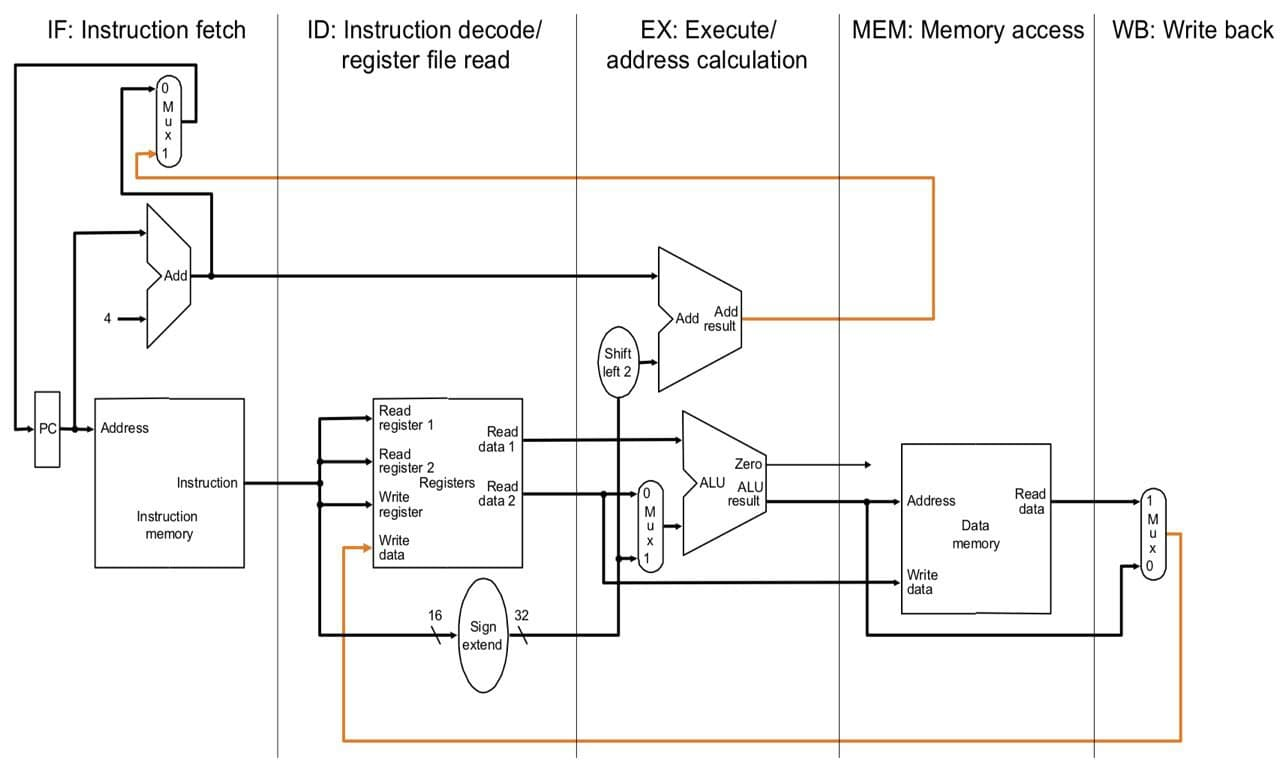
\includegraphics[width=\columnwidth]{pipelining_stage}
\end{itemize}

\textbf{{Pipeline Datapath}}
\begin{itemize}
\item Additional registers in datapath used by the same instruction between 2 stages in pipeline
\item Each pipeline register is $>$32bits
\item \textcolor{blue}{$IF$ Stage}: $IF/ID$ stores Instruction read from InstrMemory[PC] \& $PC + 4$
\item \textcolor{blue}{$ID$ stage}:
    \begin{itemize}
        \item Beginning of cycle: $IF/ID$ supplies register numbers for reading 2 registers \& 16bit offset to be sign-extended to 32bits
        \item End of cycle: $ID/EX$ stores data values read from register file \& 32bit immediate \& $PC+4$
    \end{itemize}
\item \textcolor{blue}{$EX$ Stage}:
\begin{itemize}
    \item Beginning of cycle: $ID/EX$ supplies data values read from register file \& 32bit $Imm$ \& $PC+4$
    \item End of cycle: $EX/IM$ stores $(PC+4)+(Imm \times 4)$ \& ALU result \& \texttt{isZero?} signal \& Data read 2 from register file
\end{itemize}
\item \textcolor{blue}{$MEM$ Stage}:
\begin{itemize}
    \item Beginning of cycle: $EX/MEM$ supplies $(PC+4)+(Imm \times 4)$ \& ALU result \& \texttt{isZero?} signal \& Data read 2 from register file
    \item End of cycle: $MEM/WB$ stores ALU result \& Memory read data
\end{itemize}
\item \textcolor{blue}{$WB$ Stage}:
\begin{itemize}
    \item Beginning of cycle: $MEM/WB$ supplies ALU result \& Memory read data
    \item End of cycle: Result is written back to register
    \item\textbf{Note:} \texttt{Write register} number is passed through the entire pipeline from $ID/EX$ stage until its needed in $WB$ stage\\
\end{itemize}
\end{itemize}
\columnbreak
\textbf{Different Implementations}\\
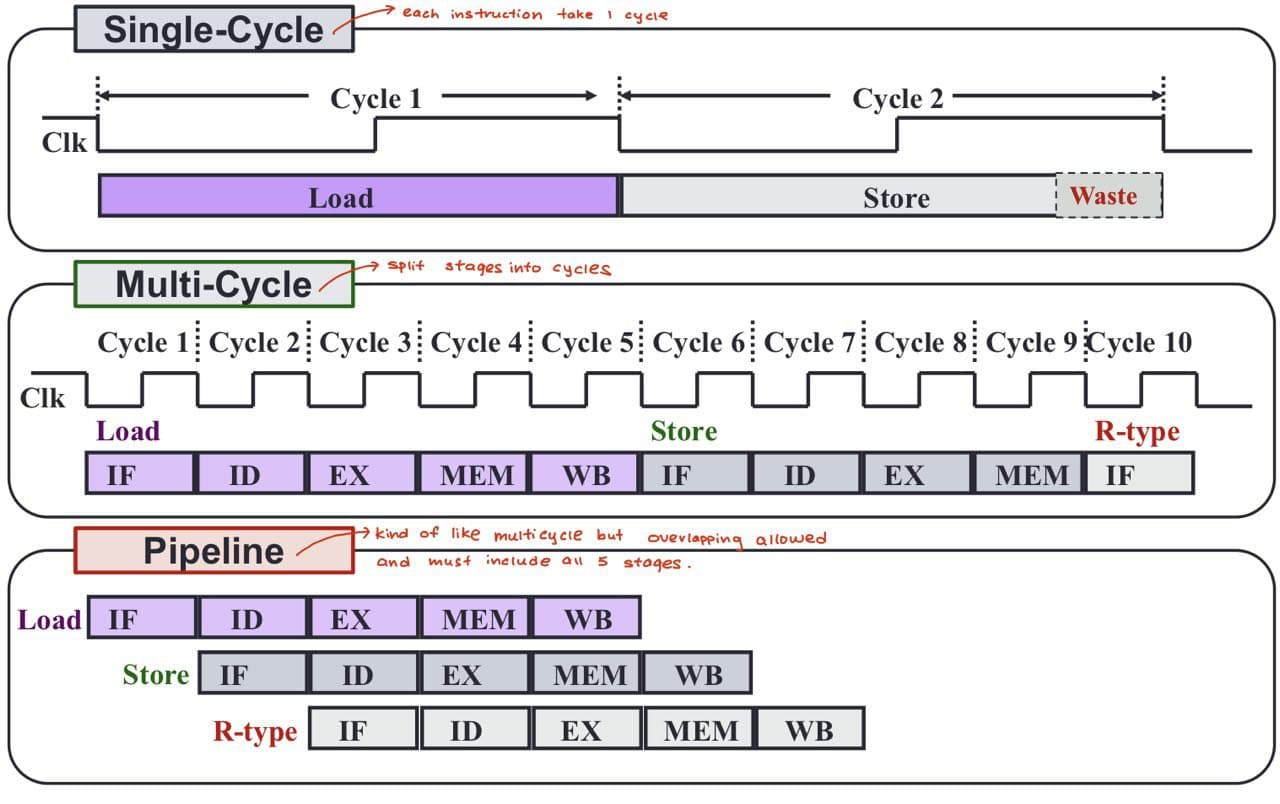
\includegraphics[width=\columnwidth]{implementations}
\textbf{{Performance}}
\begin{itemize}
\item If cycle/clock time is given, just use that
\item \textbf{Single cycle}:
    \\ Cycle time: $CT_{seq} = \text{max}(\sum^N_{k=1}T_k)$
    \\ Execution time for $I$ instructions:\\ $Time_{seq}  = I \times CT_{seq}$
\item \textbf{Multi-cycle} [1 stage per cycle, cycle time chosen to be time for longest stage]
    \\ $CT_{multi} = \text{max}(T_k)$
    \\ $Time_{multi} = I \times \textit{Average CPI} \times CT_{multi}$
\item \textbf{Pipeline} [Several stages per cycle]
    \\ $CT_{pipeline} = max(T_k) + T_d$ where $T_d$ is the pipeline register overhead
    \\ Cycles needed for $I$ instructions: \textcolor{red}{$I + N - 1$}
    \\ $Time_{pipeline} = (I + N - 1) \times CT_{pipeline}$
\item If $N_{instructions} >> N_{stages}$,
    \\ $Speedup_{pipeline} = \frac{Time_{seq}}{Time_{pipeline}} = N$ (where N is the number of pipeline stages)\\
\end{itemize}

\textbf{Hazards and resolution}\\
\textbf{Structural Hazard}:
    \begin{enumerate}[leftmargin=*]
        \item \textcolor{red}{Problem}: Single memory module will cause a clash whereby 2 instructions are accessing the memory at the same cycle.
        \\\textcolor{teal}{Solution}: Split memory into Data and Instruction memory

        \item \textcolor{red}{Problem}: Register file is accessed by 2 instructions in the same cycle
        \\\textcolor{teal}{Solution}: Split cycle into half $\rightarrow$ Write in first half, read in second half \textcolor{red}{(Order of writing/reading is important!!)}\\
    \end{enumerate}
\textbf{Data dependencies}:
\begin{itemize}
    \item \textcolor{red}{Problem}: A later instruction reading from destination register written by an earlier instruction
    \item \textcolor{teal}{Solution}: \textbf{Forwarding}
    \item Without data forwarding: If dependent instruction is
    \begin{itemize}
        \item right before: 2 cycle delay
        \item 2 cycles before \& instruction in between not dependent: 1 cycle delay
    \end{itemize}
\item With data forwarding: If dependent cycle is
    \begin{itemize}
        \item dependent on \texttt{lw}: 1 cycle delay
        \item otherwise: no delay\\
    \end{itemize}
\end{itemize}
\vfill\null
\columnbreak
\textbf{Control dependency}:
\begin{itemize}
    \item \textcolor{red}{Problem}: Incorrect execution of instructions after a branch instruction
    \item \textcolor{teal}{Solution}: \begin{enumerate}[leftmargin=*]
        \item Early branching (Make decision in $ID$ instead of $MEM$ stage
        \item Branch prediction (Assume branch \textcolor{red}{not} taken)
        \item Delayed branching (Slot in instruction with no dependencies)
    \end{enumerate}
    \item Without control measures: 3 cycle delay
    \item With early branching:
        \begin{itemize}
            \item 1 cycle delay after branch instruction
            \item With forwarding \& dependent on non-\texttt{lw}: +1 cycle delay at branch instruction
            \item With forwarding \& dependent on \texttt{lw}: +2 cycle delay at branch instruction
            \item Without forwarding \& dependent on prev instr: +2 cycles of delay at branch instruction
        \end{itemize}
    \item With branch prediction:
        \begin{itemize}
            \item 3 cycles delay if no early branching \& predict wrongly
            \item 1 cycle delay if there is early branching \& predict wrongly
        \end{itemize}
    \item With delayed branch: If $\exists$ instruction before branch that can be moved into delayed slot, move it. Else, stall/no-op\\
\end{itemize}

%CACHE%
{\small\textbf{\textcolor{blue}{Cache\\}}}
\\\textbf{Register vs SRAM vs DRAM vs Hard Disk\\}
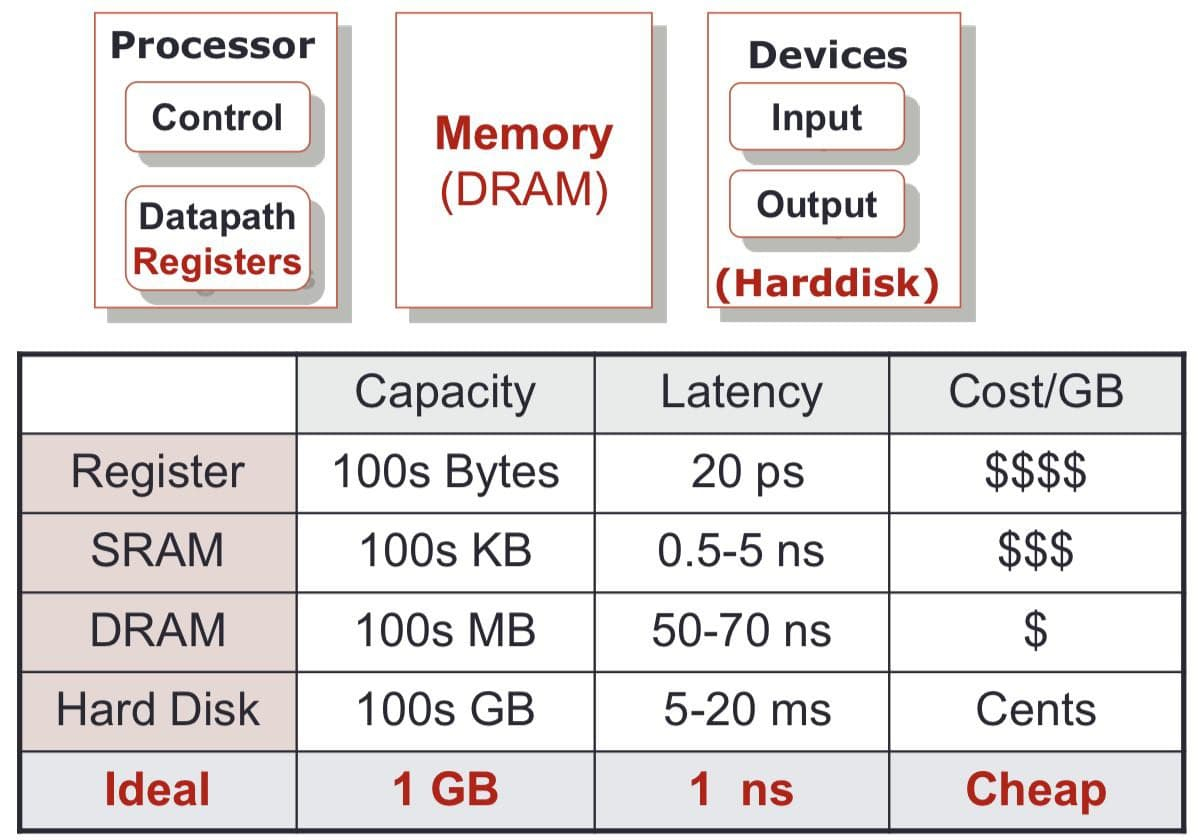
\includegraphics[width=\columnwidth]{storage}

\textbf{\\Types of locality}
\begin{itemize}
    \item Temporal locality
    \begin{itemize}
        \item If an item is reference, it will tend to be reference again soon
    \end{itemize}
    \item Spatial locality
    \begin{itemize}
        \item If an item is referenced, nearby items will tend to be referenced soon (e.g. Array access)\\
    \end{itemize}
\end{itemize}

\textbf{Terminologies}
\begin{itemize}
    \item \textcolor{teal}{Hit}: Data is in cache
    \begin{itemize}
        \item \textcolor{teal}{Hit rate}: Fraction of memory accesses that hit
        \item \textcolor{teal}{Hit time}: Time to access cache
    \end{itemize}
    \item \textcolor{red}{Miss}: Data is not in cache
    \begin{itemize}
        \item \textcolor{red}{Miss rate}: 1 $-$ Hit rate
        \item \textcolor{red}{Miss penalty}: Time to replace cache block $+$ hit time
    \end{itemize}
    \item Hit time $<$ Miss penalty\\
\end{itemize}

\textbf{Average Access time}
\\ $\text{Rate}_{hit} * \text{Time}_{hit} + (1 - \text{Rate}_{hit}) * \text{Penalty}_{miss}$\\

\textbf{{Direct Mapped Cache}}
\begin{center}
    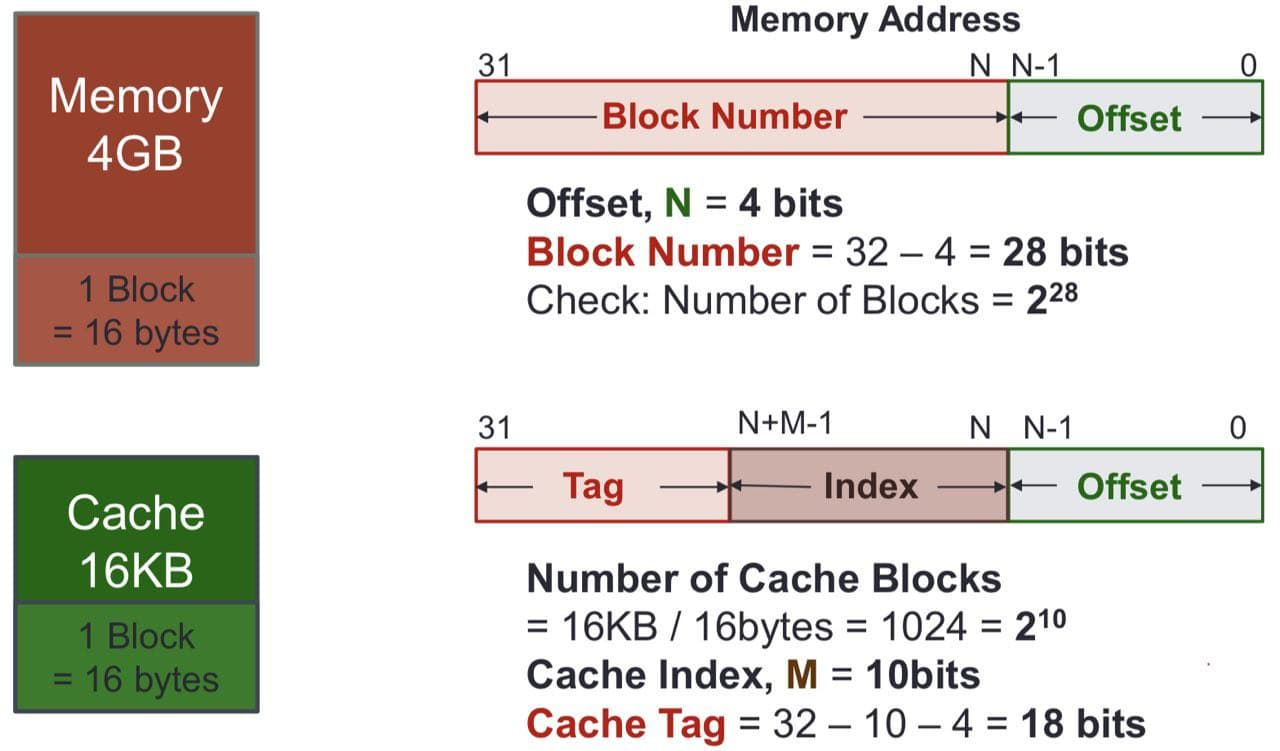
\includegraphics[scale=0.13]{direct_map}
\end{center}

\textbf{{Types of Misses}}
\begin{itemize}
\item \textcolor{red}{Compulsory misses}: On first access to a block; block must be brought into cache
\item \textcolor{red}{Conflict misses}: Occur in the case of direct mapped cache or set associative cache, when several blocks are mapped to the same block
\item \textcolor{red}{Capacity Misses}: Occur when blocks are discarded from cache as cache cannot contain all blocks needed\\
\end{itemize}

\textbf{{Writing Policy}}
\begin{itemize}
\item \textcolor{red}{Problem}: Cache and main memory are inconsistent when writing to cache
\item \textcolor{teal}{Solution}:
\begin{enumerate}[leftmargin=*]
    \item Write-through cache (Slow!)
    \begin{itemize}
        \item Write to both cache and main memory
        \item Problem: Write operates at same speed as main memory
        \item Solution: Put write buffer between cache and main memory
    \end{itemize}
    \item Write-back cache (slightly better solution)
    \begin{itemize}
        \item Only write to cache, write to memory when block is replaced
        \item Problem: Wasteful to write back to memory every time a cache block is evicted
        \item Solution: Add a \textcolor{red}{Dirty Bit} to each cache block $\rightarrow$ Write operation changes dirty bit to 1 and only write back to memory when block is replaced \& dirty bit is 1\\
    \end{itemize}
\end{enumerate}
\end{itemize}

\textbf{Handling misses}
\begin{itemize}
    \item Read miss: Load data into cache then load from cache to register
    \item Write Miss
    \begin{enumerate}[leftmargin=*]
        \item Write allocate: Load complete block into cache, change only the required word in cache, write to main memory (using write policy)
        \item Write around: Do not load block to cache, write to main memory only\\
    \end{enumerate}
\end{itemize}

\textbf{{Block size Trade-off}}
\begin{itemize}
\item Larger block size:
\begin{itemize}
    \item \textcolor{teal}{$+$} Takes advantage of spatial locality
    \item \textcolor{red}{$-$} Larger miss penalty: Takes longer time to fill up block
    \item \textcolor{red}{$-$} If block size too big relative to cache size $\rightarrow$ too few cache block $\rightarrow$ miss rate increase\\
\end{itemize}
\end{itemize}

\columnbreak
\textbf{{Set Associative Cache (SAC)}}
\begin{itemize}
\item $N$-way SAC $\rightarrow$ $N$ cache blocks per set
\item Each memory block maps to a unique cache set
\item Within the cache set a memory block can be placed in \textcolor{red}{any} of the N cache blocks
\item \textcolor{red}{Rule of thumb}: A direct-mapped cache size of \textbf{N} has about the same miss rate as a 2-way SAC of size \textbf{N/2}\\
\end{itemize}
\begin{center}
    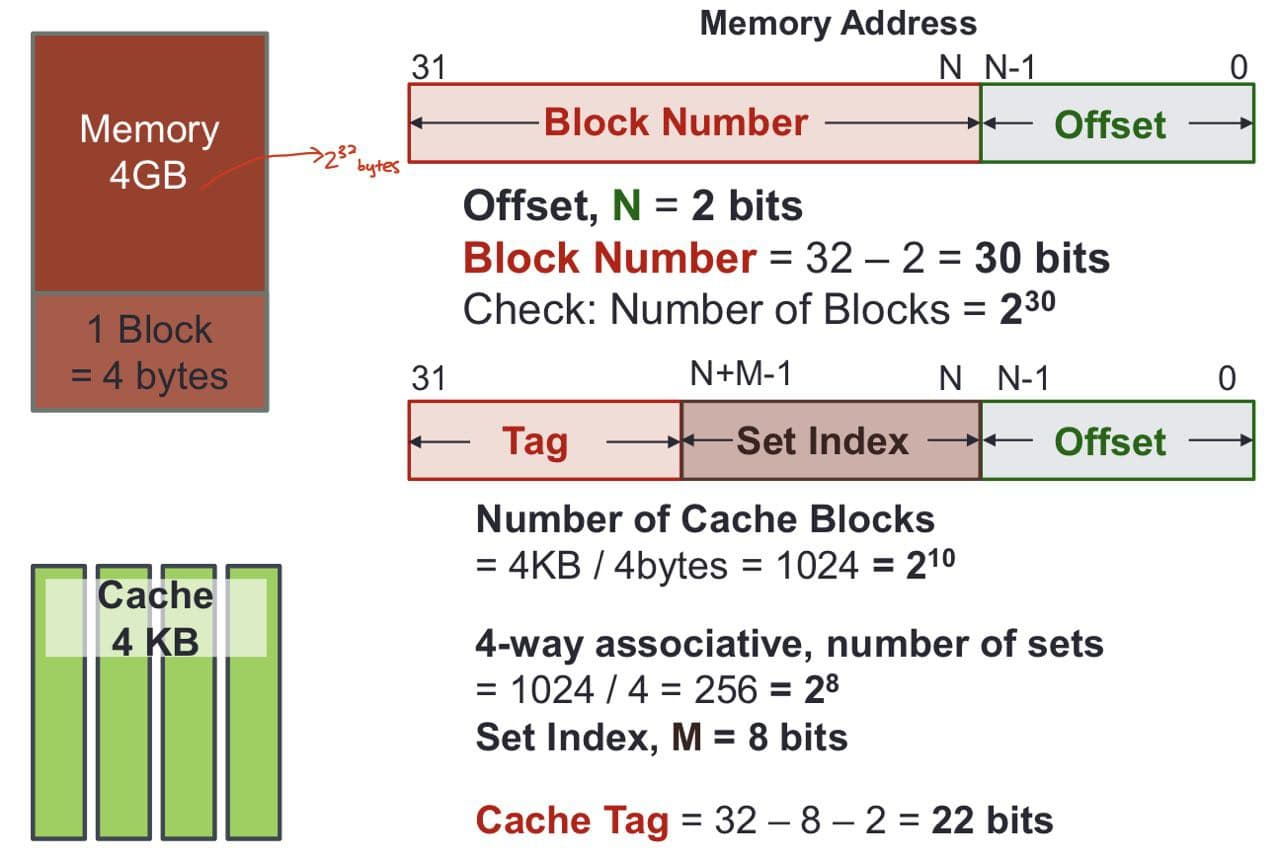
\includegraphics[scale=0.13]{SAC}
\end{center}

\textbf{{Fully Associative Cache}}
\begin{itemize}
\item Memory block can be placed in any location in the cache
\item No more cache index or cache set index
\item Need to search through all cache blocks for memory access
\item No conflict misses
\begin{center}
    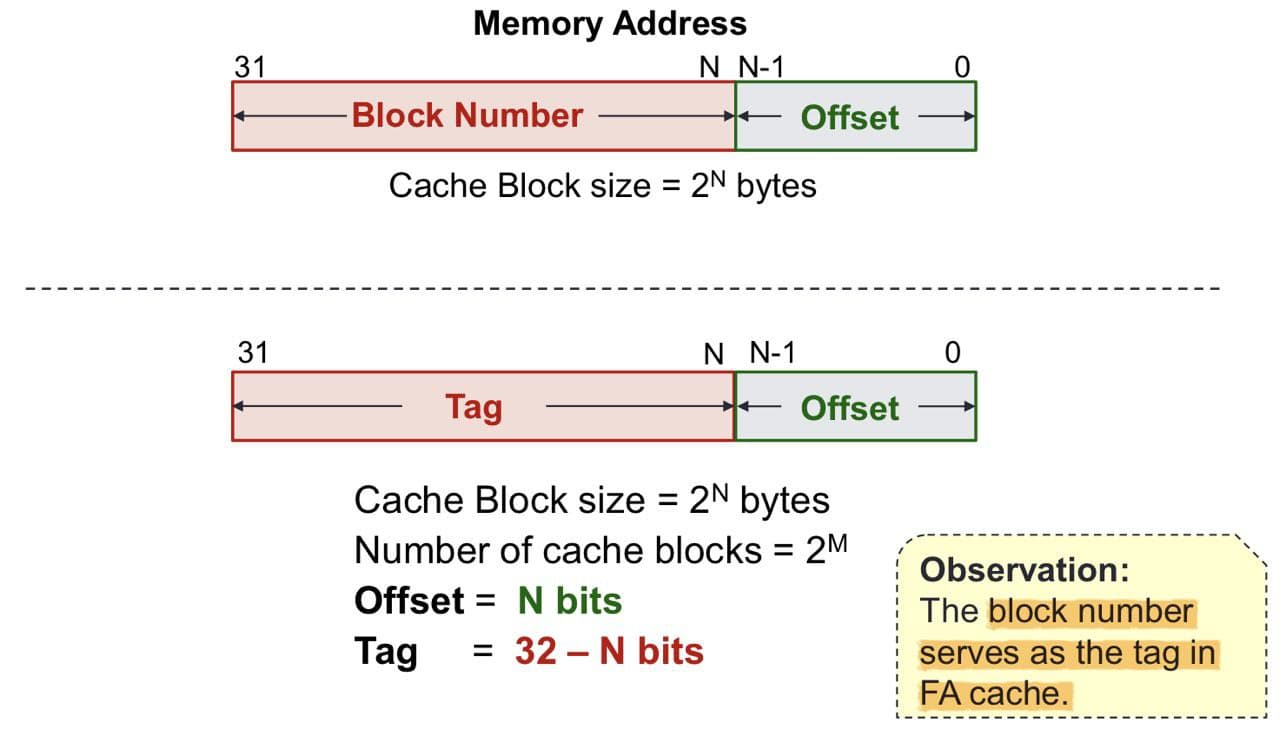
\includegraphics[scale=0.13]{FAC}
\end{center}
\end{itemize}

\textbf{{Miss Rates}}
\begin{itemize}
\item Cold/compulsory miss remains the same irrespective of cache size/associativity
\item For the same cache size, conflict miss goes down with increasing associativity
\item Conflict miss is 0 for FA caches
\item For the same cache size, capacity miss remains the same irrespective of associativity.
\item Capacity miss decreases with increasing cache size\\
\end{itemize}

\textbf{{Block Replacement}}
\begin{itemize}
\item Least Recently Used: When replacing a block, choose one which has not been accessed for the longest time (due to temporal locality)
\item First in First out
\item Random Replacement
\item Least Frequently Used
\end{itemize}

\textbf{{\\Overheads in caching}}
\begin{itemize}
\item Overheads are additional administrative information that is stored together with the data
\item Usable cache does not account for overheads
\item 3 overheads in caching: (1) Valid bit, (2) Tag of memory block, (3) Dirty bit
\end{itemize}

\vfill\null
\columnbreak
\textbf{Normal without forwarding\\}
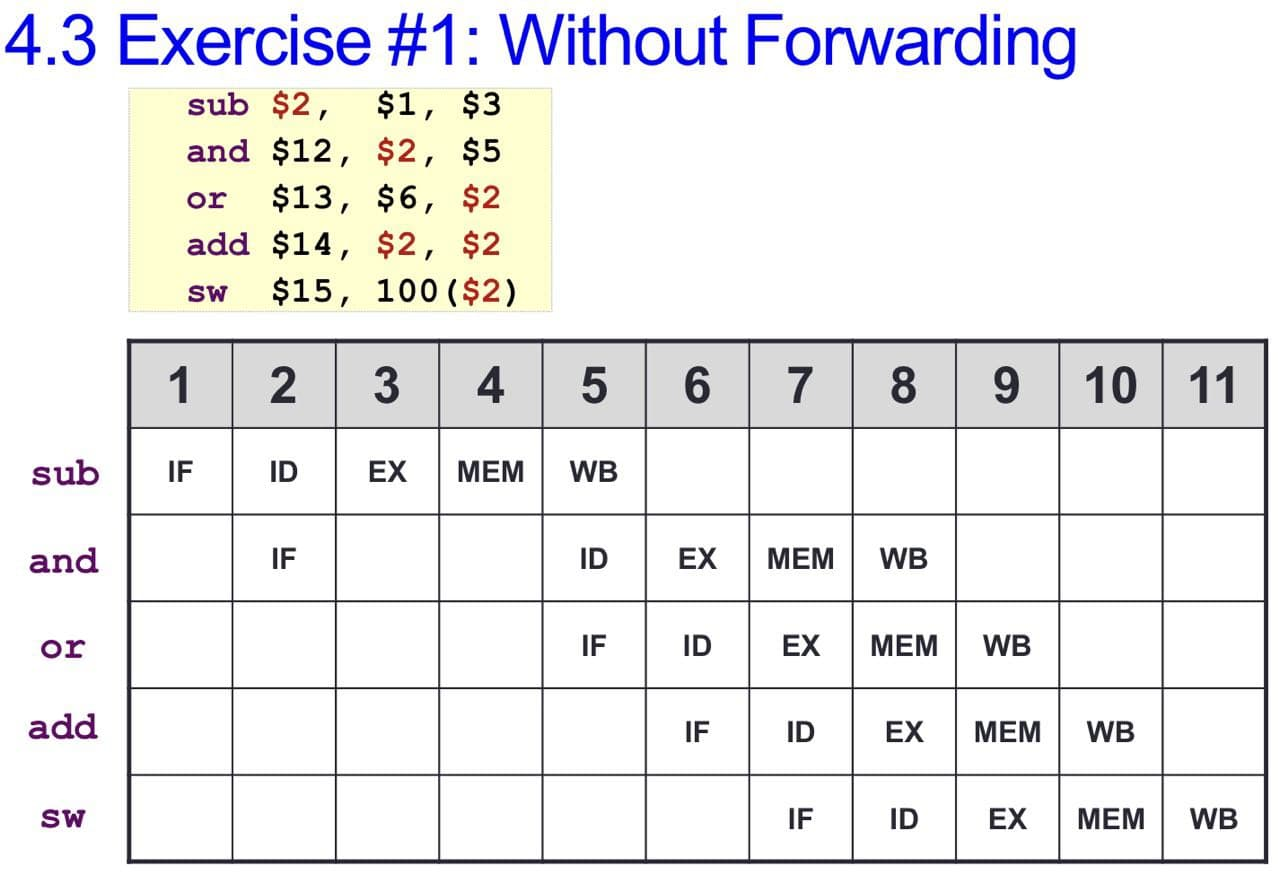
\includegraphics[width=0.90\columnwidth]{normal_without_forwarding.jpg}
\textbf{\\\\Normal with forwarding\\}
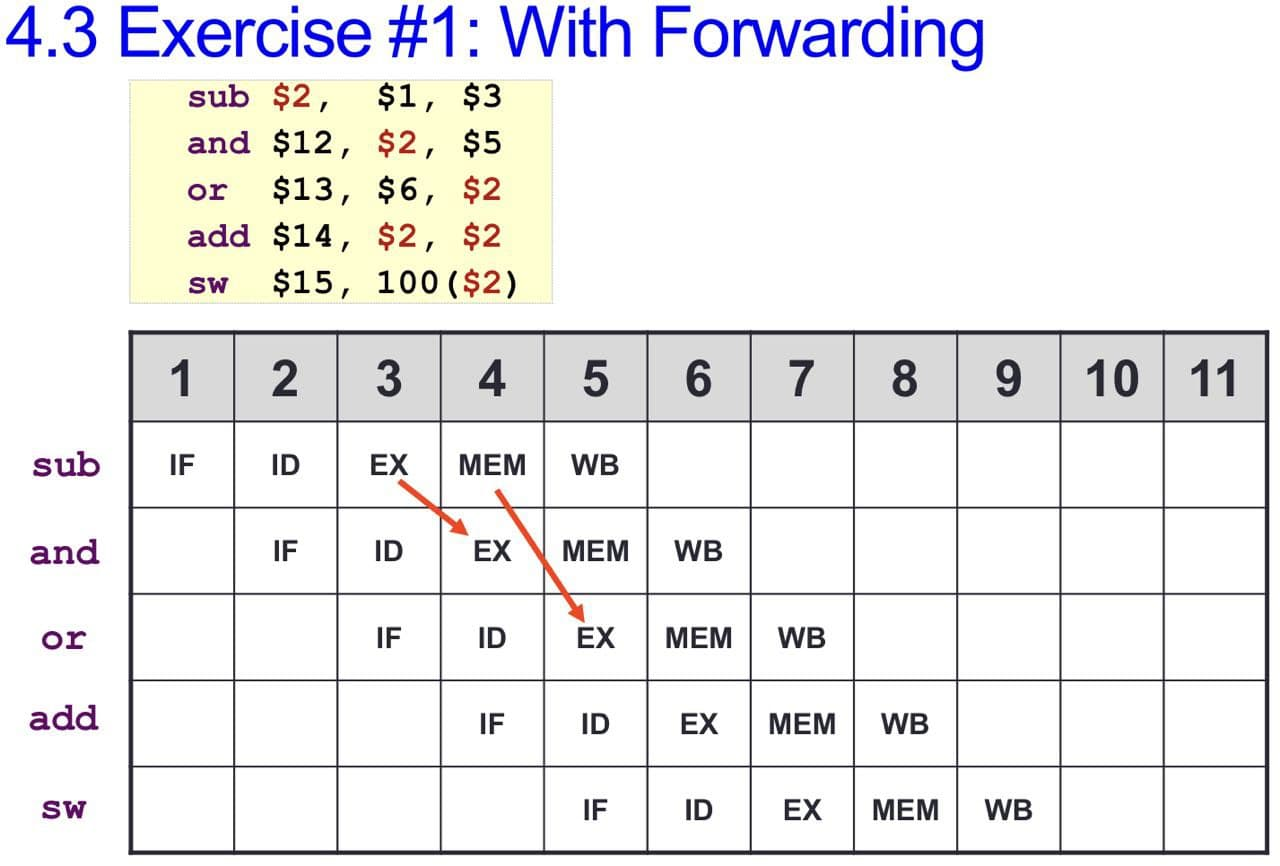
\includegraphics[width=0.90\columnwidth]{normal_with_forwarding.jpg}
\textbf{\texttt{\\\\lw} without forwarding\\}
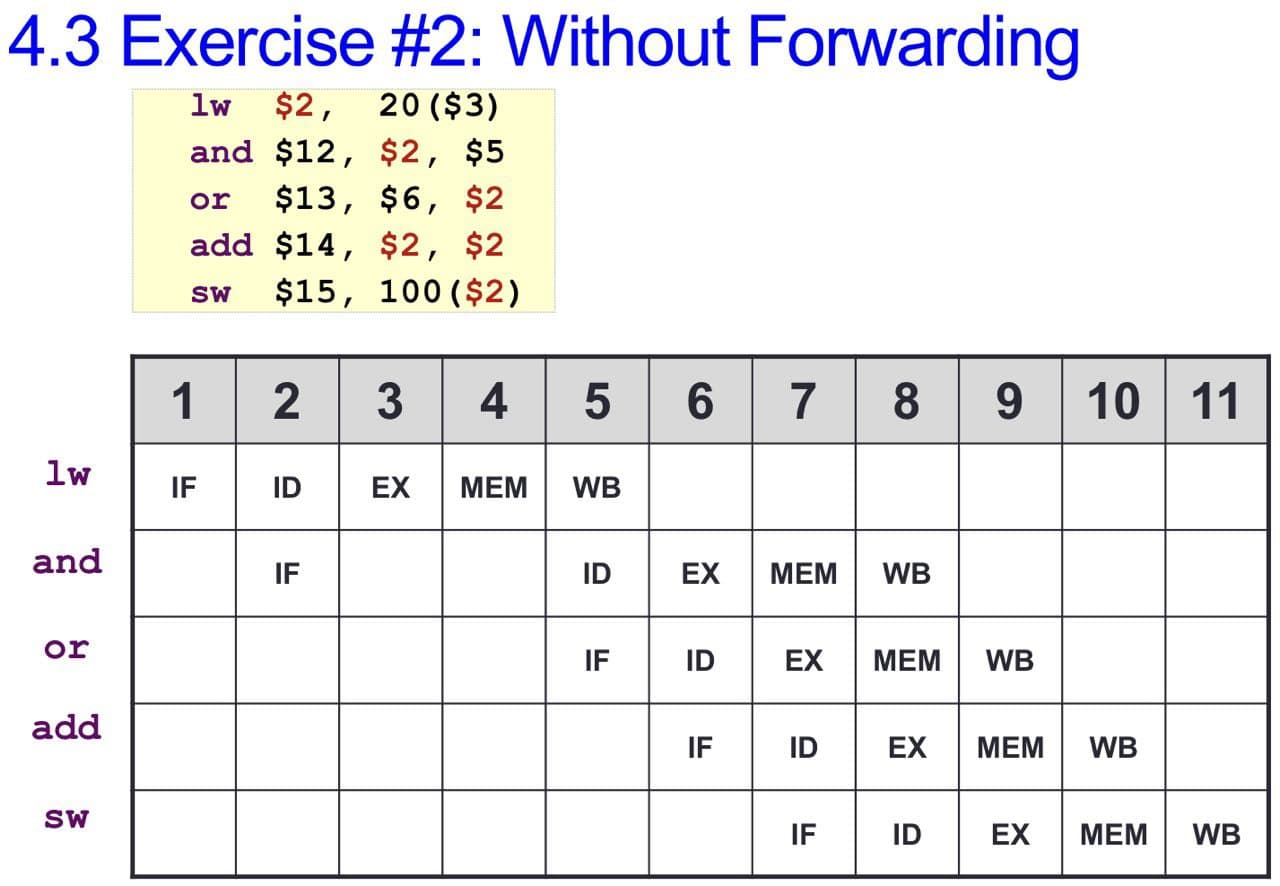
\includegraphics[width=0.90\columnwidth]{lw_without_forwarding.jpg}
\textbf{\texttt{\\\\lw} with forwarding\\}
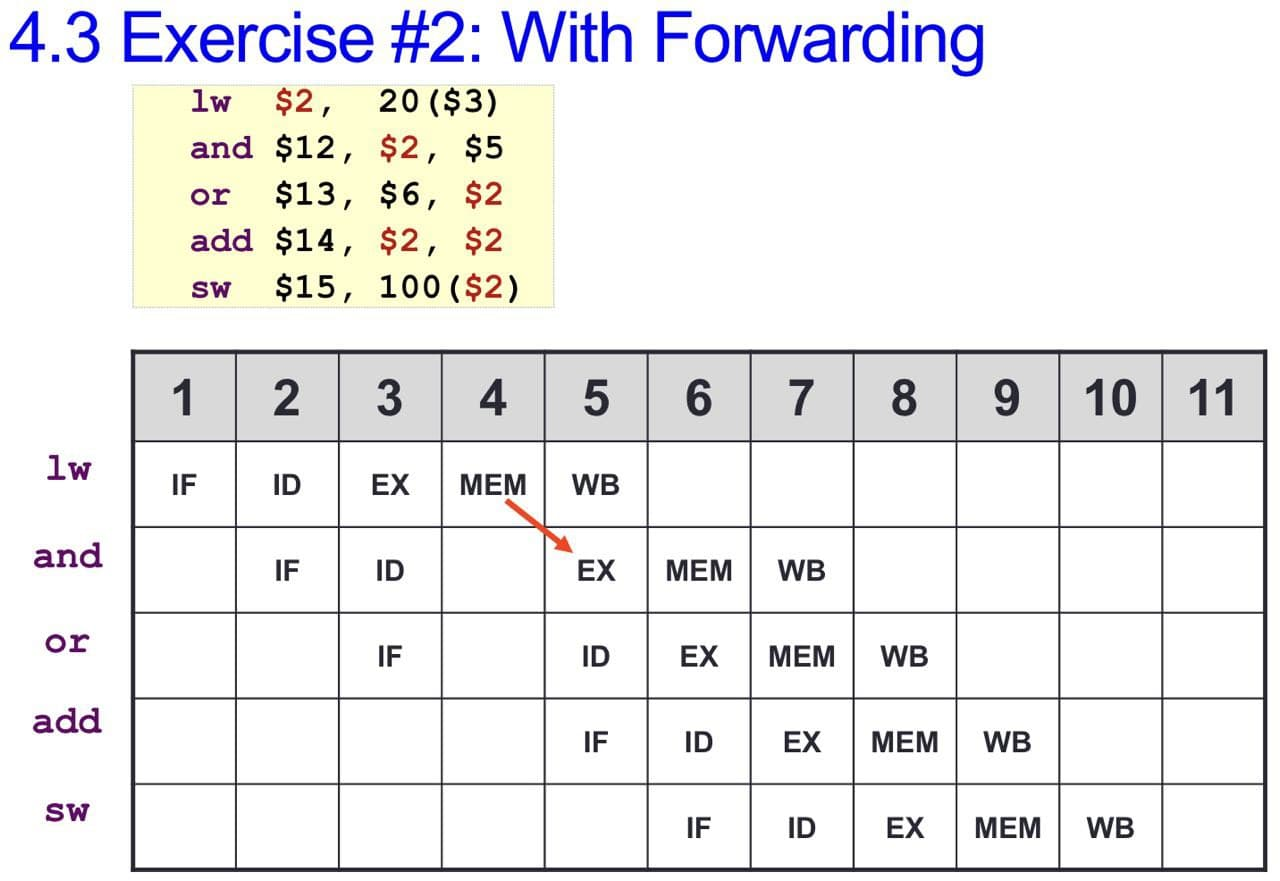
\includegraphics[width=0.90\columnwidth]{lw_with_forwarding.jpg}

\columnbreak
\textbf{Without control hazard interventions\\}
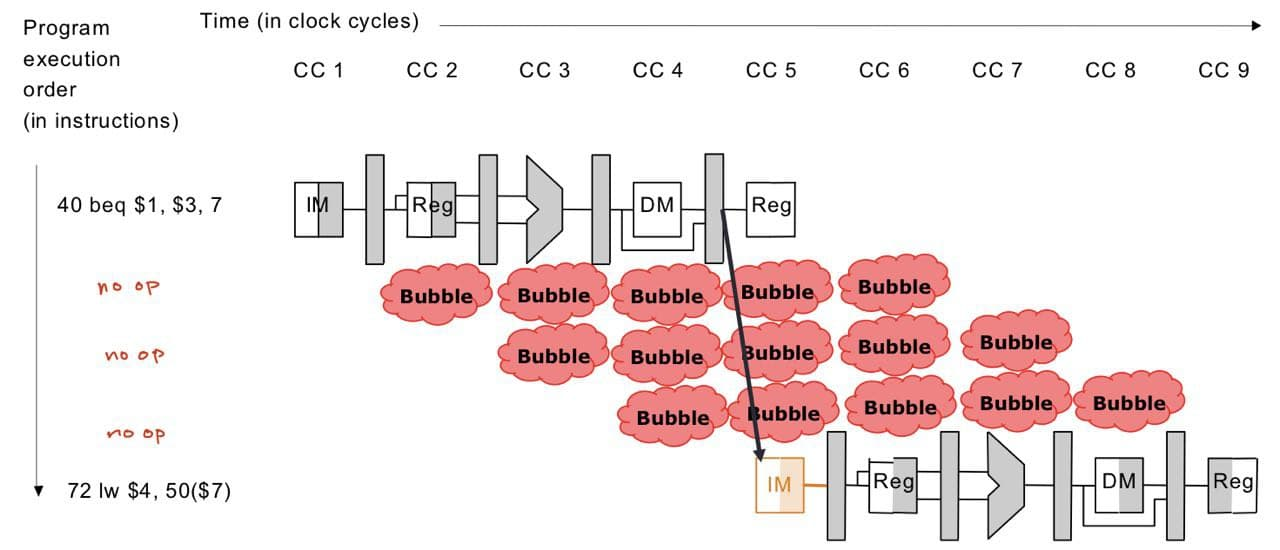
\includegraphics[width=0.95\columnwidth]{no_control.jpg}
\textbf{\\\\With early branching\\}
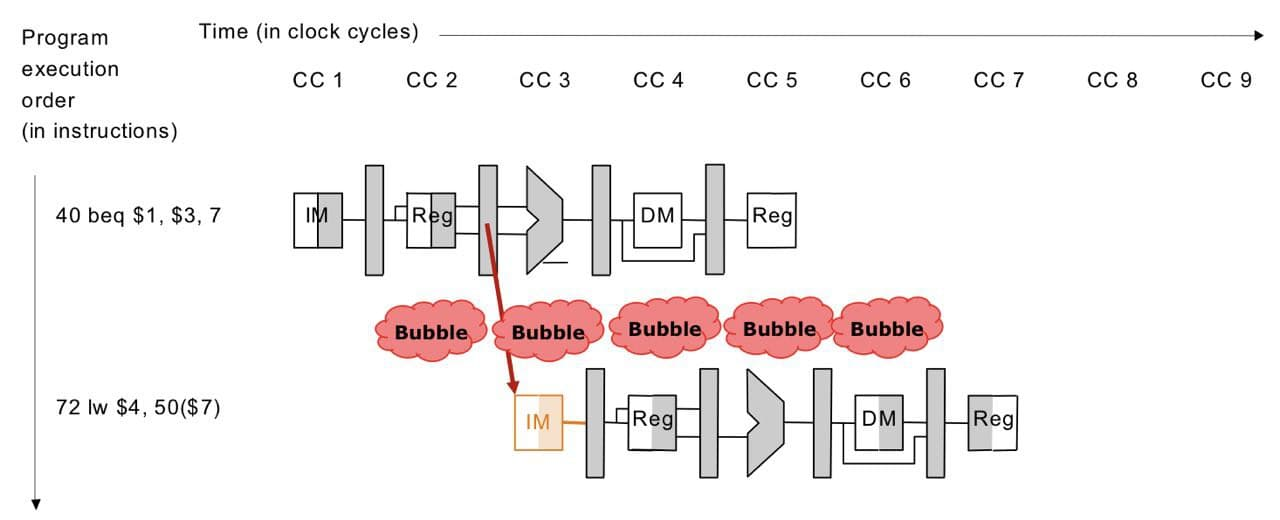
\includegraphics[width=0.90\columnwidth]{early_branch.jpg}
\textbf{\\\\Early branch with dependency \& forwarding\\}
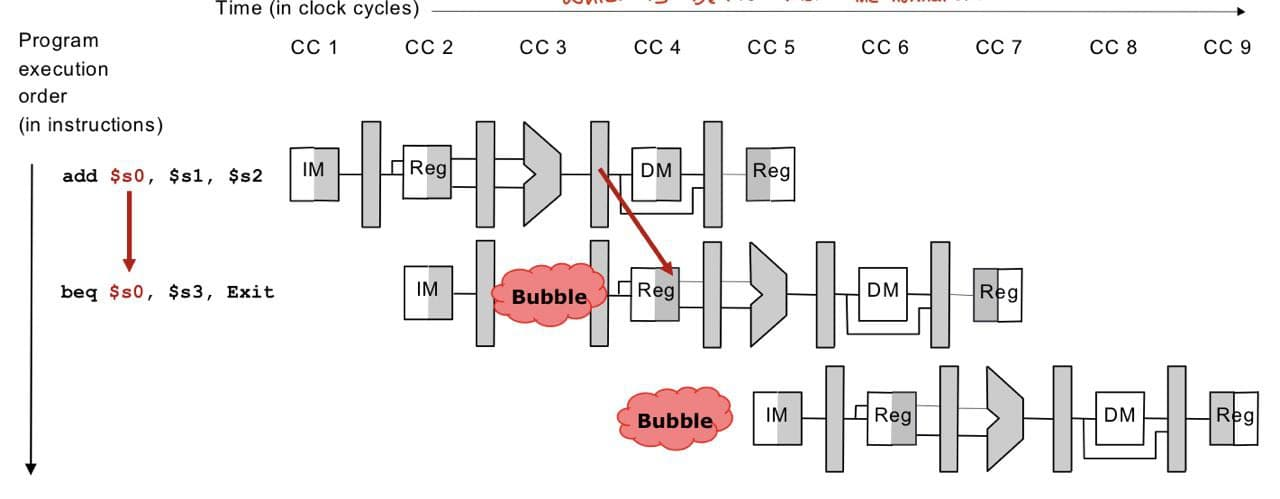
\includegraphics[width=0.90\columnwidth]{early_branch_with_dependency.jpg}
\textbf{\\\\Early branch with \texttt{lw} dependency \& forwarding\\}
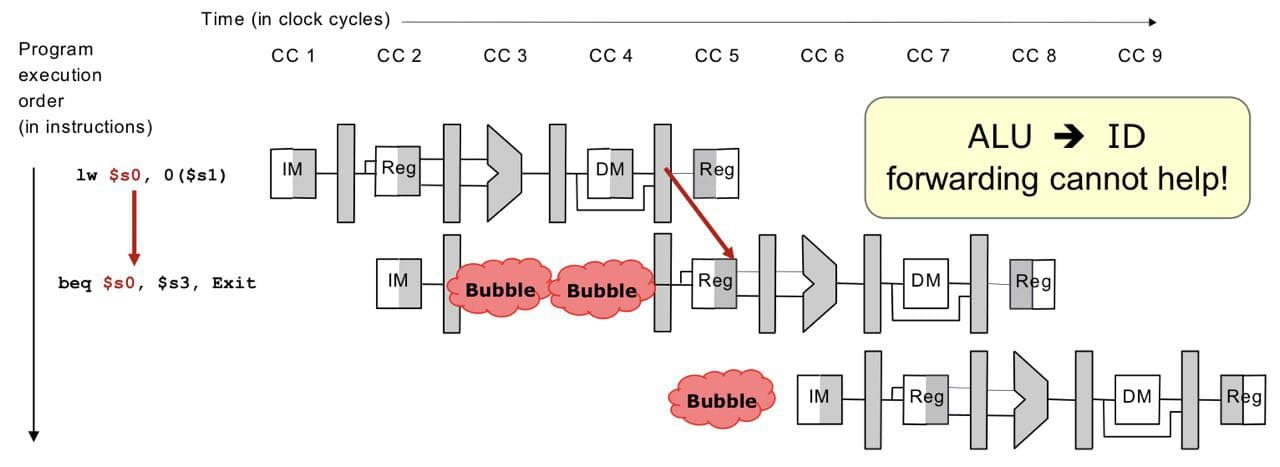
\includegraphics[width=0.90\columnwidth]{early_branch_with_lw_dependency.jpg}
% DIAGRAMS %
\vfill\null
\columnbreak
{\small\textbf{4 bit representation}}
\\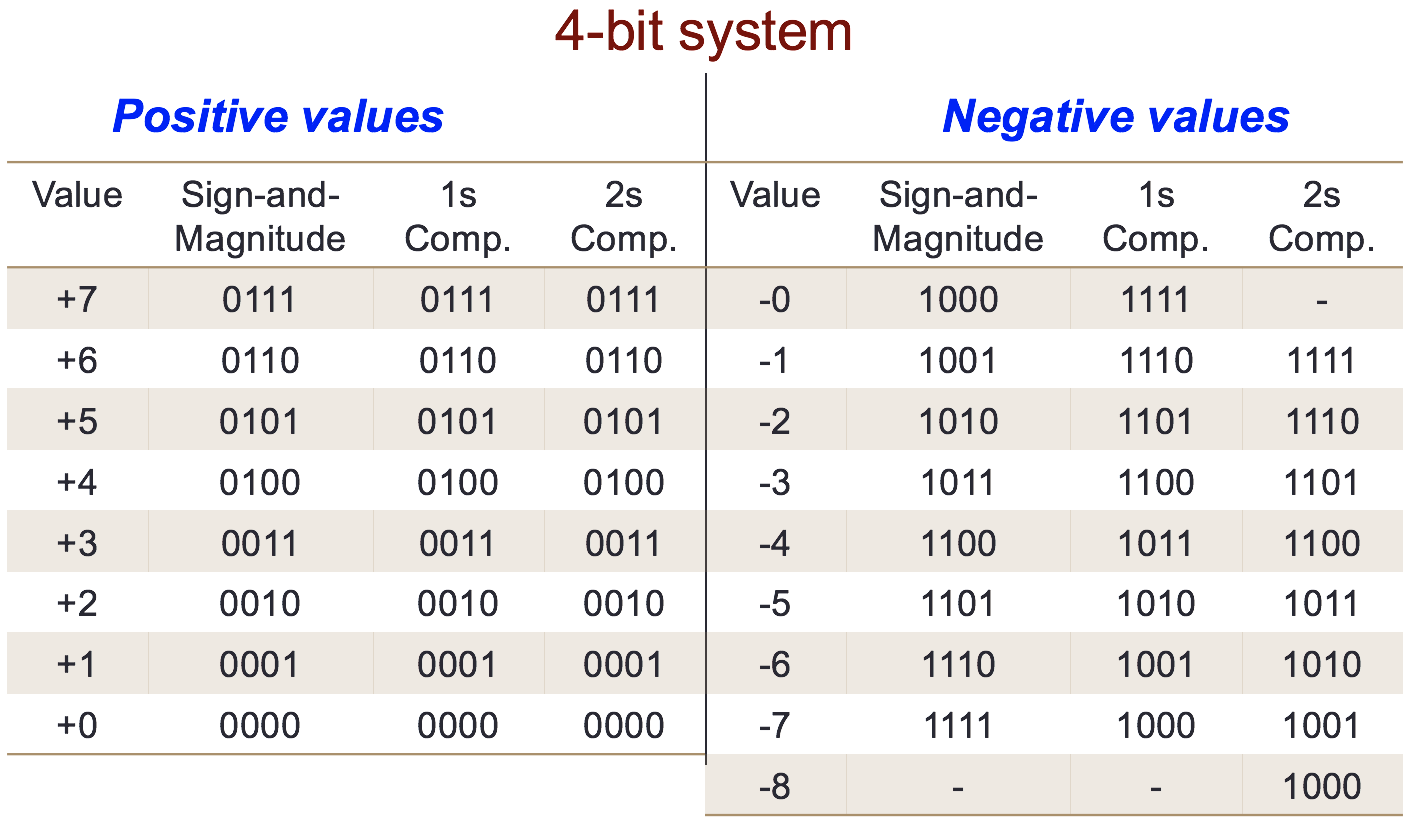
\includegraphics[width=\columnwidth]{fourBitRepresentation}\\

{\small\textbf{Pipelining control\\}}
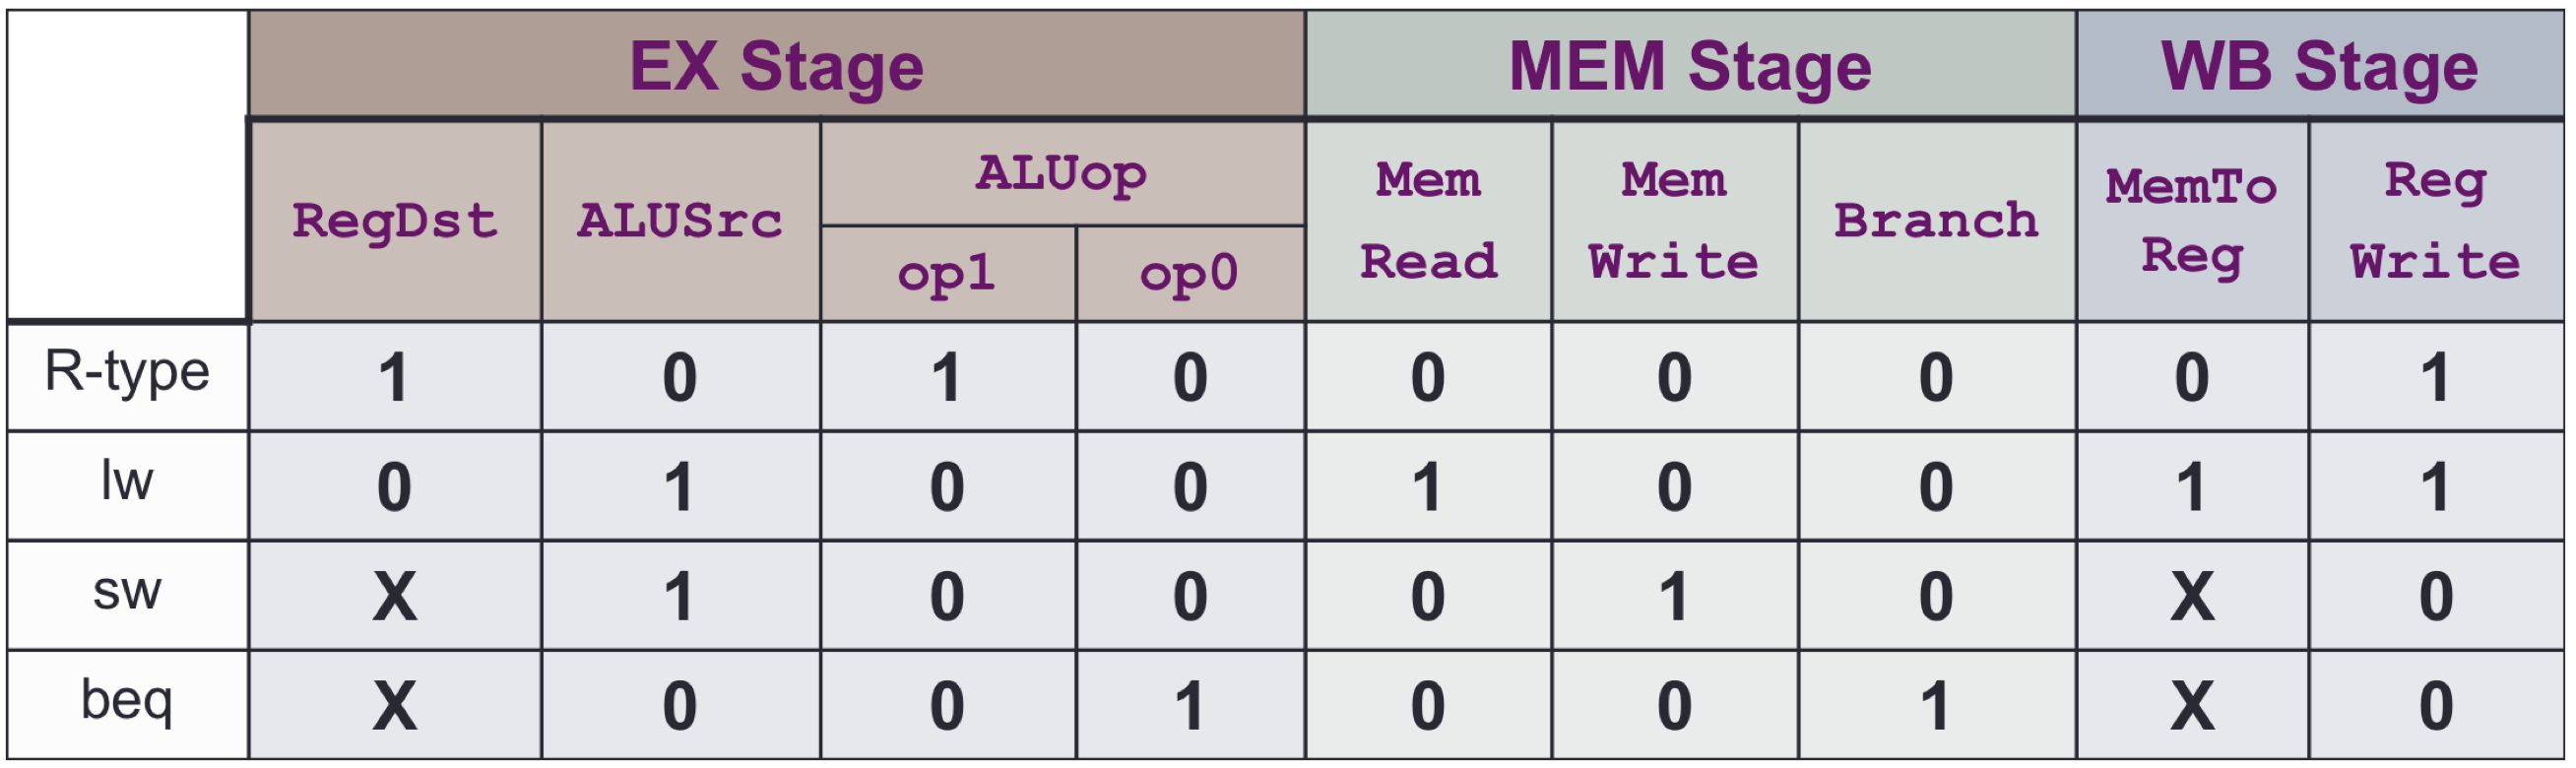
\includegraphics[width=\columnwidth]{instructionControl}\\

{\small\textbf{ALU Control Signals\\}}
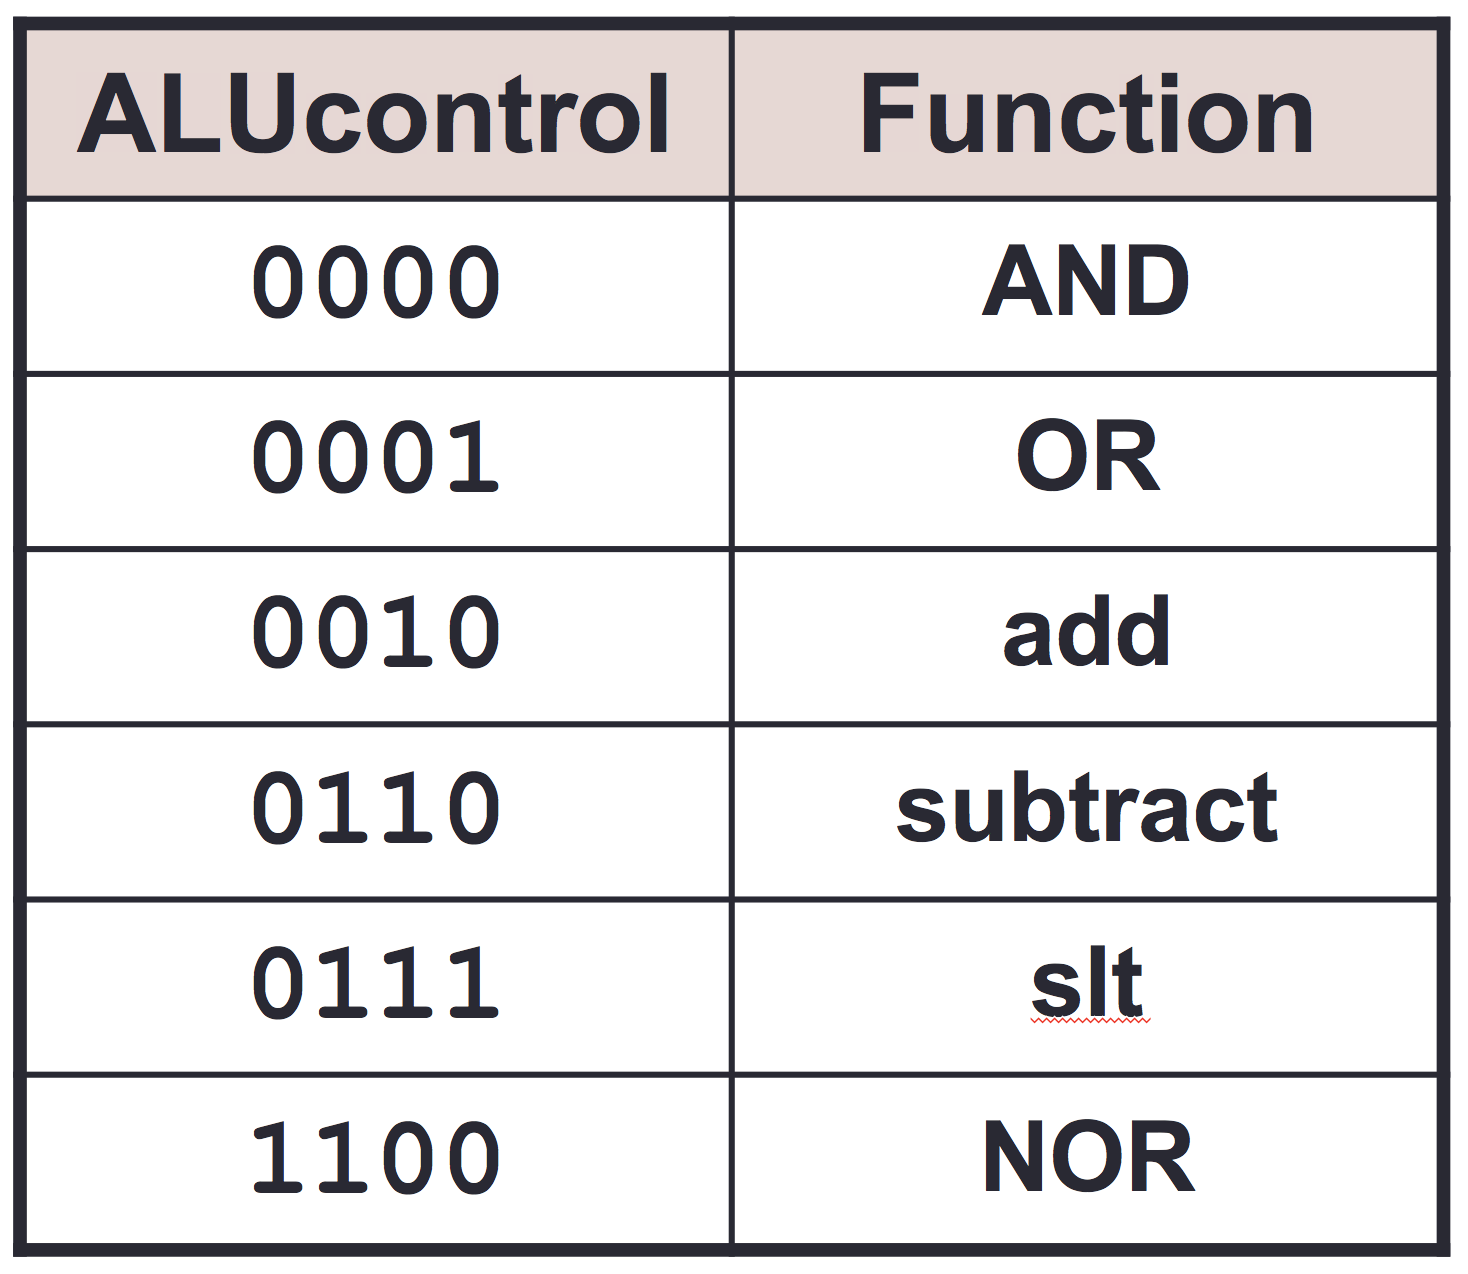
\includegraphics[scale=0.13]{ALUControl}\\

{\small\textbf{Endianness\\}}
\begin{tabular}{ |c c| }
 \hline
 Input & 0x DE AD BE EF  \\
 Big-Endian & 0: DE, 1: AD \dots  \\
 Little-Endian & 0: EF, 1: BE \dots  \\
 \hline
\end{tabular}
\vfill\null
\columnbreak
\begin{Figure}
 \centering
 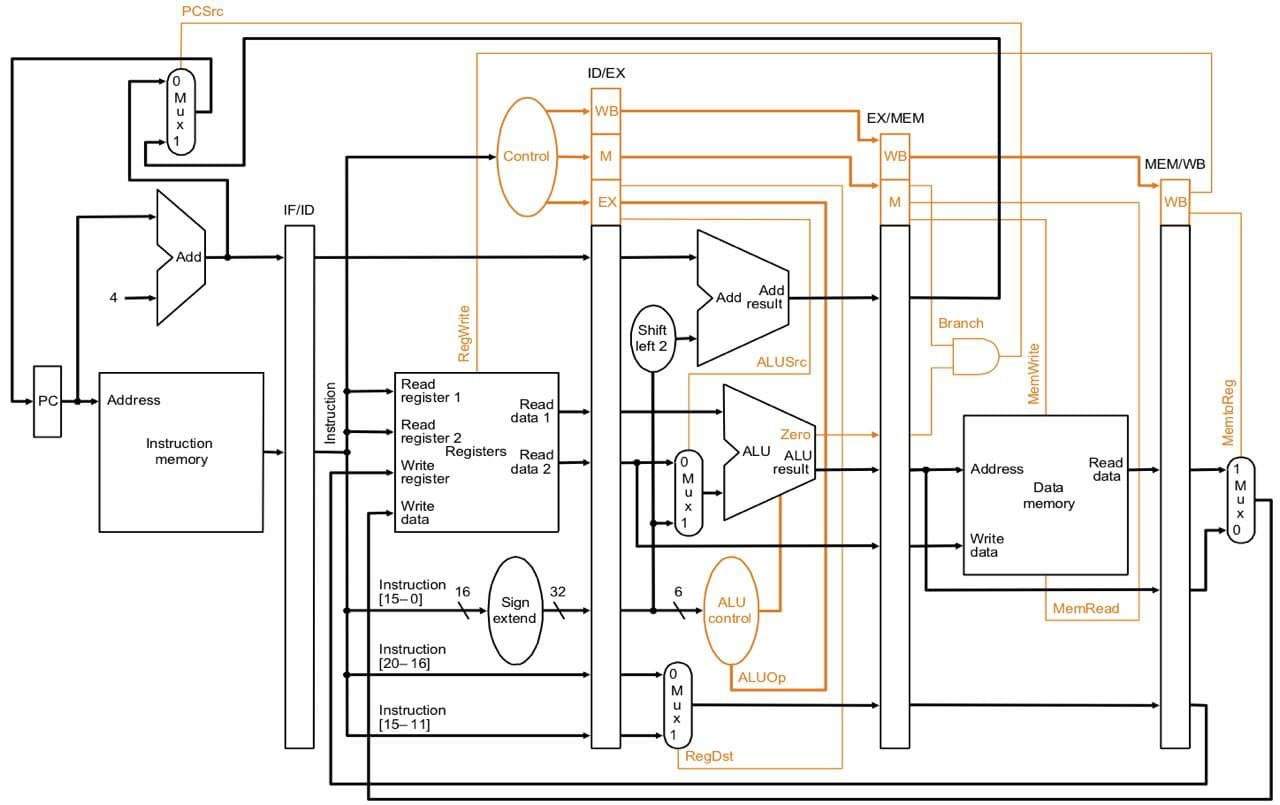
\includegraphics[angle=90, scale=0.25]{full_datapath_with_controls.jpg}
 \captionof{figure}{Datapath with pipeline control}
\end{Figure}
\end{multicols*}
\end{document}